\documentclass[11pt, a4paper, twoside]{report}

\usepackage[british]{babel}
\usepackage[useregional]{datetime2}
\DTMlangsetup[en-GB]{showdayofmonth=false} %to remove day from date
\usepackage[utf8x]{inputenc}
\usepackage[T1]{fontenc}
\usepackage{listings}
\usepackage{hyperref}
\hypersetup{colorlinks=false}
\usepackage{lscape} %to put things landscape
\usepackage{rotating} %to put things landscape, again
\usepackage{pdflscape} %trying landscape again
%\usepackage{subfigure} %removed as it was interfering with subfig package
\usepackage{amsmath} %for some maths stuff! 
\usepackage{graphicx}
\usepackage[colorinlistoftodos]{todonotes}
\usepackage{csvsimple}
\usepackage{lscape}%for landscape table in sup mat
\usepackage{apalike} %for round brackets in references
\usepackage{titlesec} %for hiding chapter title
\usepackage{subfig} % for getting 4 figures looking nice
\usepackage{setspace} %for spacing
\usepackage{listings} %for my R code
\usepackage{tikz} %for doing little circles in line with text
%\onehalfspacing %one and a half line spacing
\setstretch{1.5}
\titleformat{\chapter}[display]
  {\normalfont\bfseries}{}{0pt}{\Huge}

%%%%%This stuff is for generating tables%%%%
\usepackage{booktabs} % For \toprule, \midrule and \bottomrule
\usepackage{siunitx} % Formats the units and values
\usepackage{pgfplotstable} % Generates table from .csv

% Setup siunitx:
\sisetup{
  round-mode          = places, % Rounds numbers
  round-precision     = 3, % to 2 places
}
%%%%%%%%%%%%%%%%%%%%%%%%%%%

%% Sets page size and margins
\usepackage[a4paper,top=3cm,bottom=2cm,left=3cm,right=3cm,marginparwidth=1.75cm]{geometry}

\title{Is everything everywhere? Deterministic and stochastic processes in microbial biogeography}
\author{Amy Solman}
% Update supervisor and other title stuff in title/title.tex

\begin{document}
\begin{titlepage}

\newcommand{\HRule}{\rule{\linewidth}{0.5mm}} % Defines a new command for the horizontal lines, change thickness here

%----------------------------------------------------------------------------------------
%	LOGO SECTION
%----------------------------------------------------------------------------------------


\includegraphics[width=8cm]{logo.eps}\\[1cm] % Include a department/university logo - this will require the graphicx package
 
%----------------------------------------------------------------------------------------

\center % Center everything on the page

%----------------------------------------------------------------------------------------
%	HEADING SECTIONS
%----------------------------------------------------------------------------------------
\quad\\[1.5cm]
%\textsc{\LARGE MSc Thesis}\\[1.5cm] % Name of your university/college
\textsc{\Large Imperial College London}\\[0.5cm] % Major heading such as course name
\textsc{\large Department of Life Sciences}\\[0.5cm] % Minor heading such as course title

%----------------------------------------------------------------------------------------
%	TITLE SECTION
%----------------------------------------------------------------------------------------
\makeatletter
\HRule \\[0.4cm]
{ \huge \bfseries \@title}\\[0.4cm] % Title of your document
\HRule \\[1.5cm]
 
%----------------------------------------------------------------------------------------
%	AUTHOR SECTION
%----------------------------------------------------------------------------------------

\begin{minipage}{0.4\textwidth}
\begin{flushleft} \large
\emph{Author:}\\
Amy Solman
\end{flushleft}
\end{minipage}
~
\begin{minipage}{0.4\textwidth}
\begin{flushright} \large
\emph{Supervisor:} \\
Prof. Ryan Chisholm
University of Singapore
% Uncomment the following lines if there's a co-supervisor
%\\[1.2em] % Supervisor's Name
%\emph{Co-Supervisor:} \\
%Dr. Adam Smith % second marker's name
\end{flushright}
\end{minipage}\\[3cm]
\makeatother


%----------------------------------------------------------------------------------------
%	DATE SECTION
%----------------------------------------------------------------------------------------

{\large A thesis submitted for the degree of}\\[0.5cm]
{\large \emph{MRes Computational Methods in Ecology and Evolution}}\\[0.5cm]
{\large \today}\\[2cm] % Date, change the \today to a set date if you want to be precise

\vfill % Fill the rest of the page with whitespace

\end{titlepage}

\renewcommand{\abstractname}{Declaration}
\begin{abstract}
\textbf{Concept:} The concept for this work came from Prof. Thomas Bell and Prof. Ryan Chisholm.\\
\noindent \textbf{Data:} All data for this analysis was collected by myself from the literature as listed in the Supplementary Materials section.\\
\noindent \textbf{Simulation:} All simulation code was written by myself, excluding function 2: coalescence\_test (simulation scripts) provided by Dr. James Rosindell.\\
\noindent \textbf{Model:} The Classic, Depth and Perimeter models, as well as critical area formulas, were supplied by Prof. Ryan Chisholm.\\
\noindent \textbf{Analysis:} I declare that all analysis was carried out by myself.\\
\noindent \textbf{Report:} I declare that the report was written by myself.\\
\\ \\ \\

\noindent \textbf{COVID-19} \\
\noindent The hypotheses presented in this report were originally investigated using a laboratory-based experiment in Professor Thomas Bell's Microbial Ecology Laboratory, Imperial College London, Silwood Park. Two months into the investigation, laboratory work was ceased due to the COVID-19 pandemic. The following report seeks to test the same hypotheses, using data from the literature.
\end{abstract}

\renewcommand{\abstractname}{Abstract}
\begin{abstract}
1. Microbial communities play an essential role in biogeochemical processes and ecosystem functioning. Despite their importance, relatively little is known about the mechanisms driving spatial scaling within these communities. \\

\noindent 2. The Theory of Island Biogeography predicts that species richness increases with island area through stochastic colonisation-extinction processes. It has been widely use to describe macroorganism spatial patterns, with little application to microbial communities.\\

\noindent 3. Despite the popularity of this theory, small islands often show no clear relationship between species richness and area. Chisholm \textit{et al.,} have addressed this by developing a unified theory of species-area relationships that transitions from a niche-structured regime at smaller spatial scales to stochastic mechanisms at larger spatial scales.\\

\noindent 4. This work modifies the Chisholm model to address microbial communities in a range of habitats. Through model fitting I assess to what extent microorganisms are subject to deterministic or stochastic processes. I also explore how the transition between regimes differs among habitat types and taxonomic groups. \\

\noindent 5. The models gave good fits to the data. Multiple regression analysis showed significant evidence that taxonomic group explained variance in the critical area of transition between regimes. Less motile groups exhibited higher critical areas supporting my hypothesis. Habitat type was non-significant in predicting critical area.\\

\noindent 6. A proportion of the datasets exhibited a biphasic species-area relationship. Broadly the critical area hypotheses of lower transition areas for more motile taxa was supported by the data. These results can assist in predicting the spatial scaling of microbial diversity, with application to climate change modelling. \\

\noindent \textbf{Keywords:} species-area relationships, taxa-area relationships, microbial biogeography, small-island effect, niche structure, colonisation-extinction balance, island biogeography
\end{abstract}

\tableofcontents
\listoffigures
\listoftables

\chapter{Introduction}

MacArthur and Wilson's theory of island biogeography \cite{MacArthurRobertH1967Ttoi} is widely accepted as a fundamental ecological law. It posits that island communities are maintained by a combination of immigration and niche availability. Niches provide reduced inter- and intraspecific competition, slowing competitive exclusion. Immigration provides new species and new individuals, offsetting loses to competitive exclusion and genetic drift. Islands with a larger area and reduced distance from mainland communities or other islands, will exhibit higher species diversity at colonization-extinction dynamic equilibrium than those smaller and further away. A great deal of empirical evidence has been amassed to support the theory of island biogeography and it has been widely applied in understanding the effects of habitat fragmentation \cite{haila2002conceptual}. \

\indent Despite the popularity of this theory, there is empirical evidence to suggest it cannot always be applied to smaller islands \cite{triantis2006re}\cite{sfenthourakis2009habitat}. MacArthur and Wilson noted that archipelagos showed unusual SARs, with smaller island species-richness varying independent of size \cite{MacArthurRobertH1967Ttoi}. This exception to MacArthur and Wilson's putative ecological law has been dubbed the small island effect (SIE). Several hypotheses have been offered to explain the SIE. The 'subsidized island biogeography' (SIB) hypothesis suggests that smaller islands have a greater edge:interior ratio, thus receive a greater amount of nutrients per unit area in contrast to larger islands \cite{barrett2003small}\cite{anderson2001subsidized}. Moreover, extinction rates on islands may operate independently of area due to their environmental instability and high temporal turnover, where major episodic disturbances periodically wipe out colonizing species \cite{chisholm2016maintenance}. Thirdly, the 'habitat hypothesis' suggests a limited suite of habitats on small islands, in contrast to larger islands, limits species diversity \cite{triantis2008evolutionary}. \

\indent Chisholm \textit{et al} \cite{chisholm2016maintenance} have developed a unified theory to explain this biphasic island SAR. They posit that this pattern of species-richness is due to a transition from a niche-structured regime on smaller islands, to a colonization-extinction regime on larger islands. The niche-structured regime is characteristic of deterministic niche theories where environmental filtering, biotic interactions and interspecific trade-offs determine species richness \cite{chase2011disentangling}. The colonization-extinction regime is characteristic of stochastic theories such as the theory of island biogeography and neutral theory, where richness is dictated by colonization and extinction rate as well as ecological drift \cite{hubbell2001unified}.\

\section{Microbial Communities}

\indent Whilst numerous studies have looked at macro-organism SARs, relatively little is known about how microbial species are affected by habitat size, isolation and niche availability. Understanding the factors that regulate microbial species richness and community structure is important as they play a significant role in ecosystem functioning \cite{griffiths2011bacterial}. Greater understanding of the patterns underlying microbial biogeography is also important in predicting the responses of these organisms to a changing environment \cite{bradley2017microbial}.\

\indent Debate around the applicability of SARs to microbial systems stems from the idea that they are ubiquitous in the environment and functionally redundant. This was famously articulated by Bass-Becking \cite{baas1934geobiologie} who wrote, 'everything is everywhere, but, the environment selects'. Some studies have shown that SAR theories are not useful in describing microbial richness patterns \cite{fierer2006diversity} \cite{henebry1980effect}. \

\indent Investigating microbial biogeography also has its practical challenges. Problems often arise in experimentally manipulating habitats to a degree useful for such a study and it is only recently that advances in molecular tools has lead to a resurgence in the field. One study found bacterial SARs in aquatic treehole habitats comparable with that of larger organisms \cite{bell2005larger}. Organic aggregates have also been used as 'islands' to explore the biogeography of aquatic pathogens \cite{lyons2010theory}, showing a weak positive correlation between ‘island’ size, community metabolic response and functional diversity. Investigation of phytoplankton SAR in water bodies found evidence for the SIE, however they also detected a large lake effect where species richness declined beyond a threshold area as wind-induced mixing increased habitat homogeneity \cite{varbiro2017functional}. This indicated that small-scale niche relations were the most important determinants of species richness at the smallest spatial scales. The SIE has also been seen in benthic diatoms sampled from ponds on a wide spatial scale \cite{bolgovics2016species}. Increased niche dimensionality has been shown to increased functional diversity, with strong evidence for niche filtering of microbial taxa communities \cite{KevinLee2016Nfob}.\

\indent The majority of studies looking at microscopic island biogeography have focused on aquatic communities. This is likely due to the availability of isolated water bodies and their range of spatial scales. Bacteria also represent a major contributor to soil biodiversity and processes \cite{griffiths2011bacterial}. Despite this, little is known about belowground regulators of biodiversity. An in-situ study of ectomycorrhizal fungi communities within 'tree island' root systems showed that total species richness increased significantly with island size, but distance had little effect \cite{peay2007strong}. Despite the strong SAR found in this study, there was no good evidence linking the SAR to increases in niche variety with habitat size, a result consistent with the theory of island biogeography and neutral community models. Most investigations have manipulated habitat area only, inferring that niche availability will naturally vary with habitat size. One study directly manipulated niche dimensionality by varying resource richness and found this resulted in increased functional dissimilarity, community productivity and reduced invasion \cite{eisenhauer2013niche}. \

\indent To tackle the limitations of previous in-situ research where environmental variables were difficult to control \cite{fenchel2005bacteria}, this study aims to quantify the contributions of immigration and niches to diversity in a soil microbial community, by manipulating mesocosm 'island' habitats. We aim to assess whether Chisholm's unified theory of biphasic island SARs is supported by our results. The parsimonious machanistic model used by Chisholm \textit{et al} \cite{chisholm2016maintenance} to approximate the processes of a biphasic SAR is fit to the data, along with other mathematical models. The number of microbial species maintained by niches is inferred from the asymptotic richness as immigration rates are reduced. The contribution of immigration is inferred from the rate of richness increase across treatments. This investigation seeks to identify nonlinearities in the richness versus immigration curve. \

\section{Hypotheses}

\indent It is hypothesise that: \ 

1) Soil microbial communities will be dictated by a niche-structure regime at the smallest spatial scales, before transitioning to a colonization-extinction regime at larger spatial scales. \

2) 'Islands' with lower rates of immigration will have less species at the colonization-extinction dynamic equilibrium. \

\chapter{Methods}
The model fitting process was validated by developing a simulation from which parameters of theta, migration rate and niches could be retrieved. A specifically designed laboratory experiment was commenced in January 2020 to test the model's theories in relation to microbial community dynamics. Due to the COV-19 pandemic the laboratory experiment was ended in March 2020. An alternative approach was devised, in which the model was fit to microbial species-area datasets compiled from the literature.

\section{Laboratory Experiment}

\subsection{Study area and sample collection}
\noindent

Soil was collected on site at Silwood Park, Berkshire, UK. Silwood Park comprises a variety of habitats including woodland, wetlands, heathland and formerly arable land \cite{CrawleyMichaelJ2005TfoB}. Soil types across the site consist of sandy or silty loam, with pH ranging from 4 to 6 \cite{LuckettKathryn2015Tbfr}. For this experiment soil was collected from a fallow field of acidic, sandy soil \cite{CrawleyMichaelJ2005TfoB}. Samples were acquired and sterilised during the first week of February. A total of 100 litres of soil was collected.

\subsection{Preparation of soil and mesocosms}
\noindent
The soil was homogenised by sieving and sterilising three times using an autoclave to destroy any present bacteria or fungi. We used five sizes of container: 0.2ml (PCR tube), 1.5ml (Eppendorf), 50ml (Fallon), 500ml and 5000ml. For each size of container 1, 2, 3, 4, 5 and maximum number of holes were made using a heated needle. Three replicates were made for each size of container and number of holes. The containers were then sterilised using the autoclave. The containers were filled with sterilised soil and sealed with an opaque lid. The containers were then buried on site, with sealed lids exposed and left to incubate for one month. 1.	If we use transparent covers for the tops of the tubes/containers this may create a gradient of light energy and moisture? Provide niches for heterotrophic and phototrophic microbes? Niche-based processes have been shown to be predominant in structuring observed aridity-related community patterns \cite{HuangMuke2019Iaas}. Abundance of predatory myxobacterial communities has also been correlated with temperature \cite{ZhouXiu‐Wen2014Mcia}.

\subsection{Soil properties measurements and climate data collection}
\noindent What is the pH of the soil where the samples were collected? pH of the soil where the samples were buried? pH has been show to affect microbial diversity \cite{GriffithsRobertI.2011Tbbo}.

\subsection{DNA extraction and sequence analysis}
\noindent After one month the containers were retrieved and DNA sampling was carried out the ZR Fungal/Bacterial DNA MiniPrep™ Isolation kit. Estimation of relative abundances of bacterial taxonomic groups was carried out using a previously defined PCR-based method \cite{FiererNoah2005Aosm}. Real-time PCR, or qPCR, allows for rapid quantitative assessment of soil microbial communities. I used 388 forward primer and 518 reverse primer as suggested for targeting all bacterial groups \cite{FiererNoah2005Aosm}. DNA samples from all 90 mesocosms were prepared for Illumina MiSeq 16S sequencing.

\section{Simulation}

\subsubsection{Overview}
This simulation is designed to mimic the process of island colonisation from a metacommunity. The colonisation process is constrained by migration rate and each island is characterised by number of niches and the size of each niche. The output of the simulation is the final community in each niche of each island, as well as a timeseries of species richness. 

\subsubsection{Metacommunity}
A metacommunity is generated at the beginning of the simulation using \textit{coalescence\_test} function, partially modified from a script provided by Dr James Rosindell. The function takes the input parameters: metacommunity size(\textit{J\_meta} = 50 000) and speciation rate (\textit{nu} = 0.001). Each run of the function produces 20 niche communities, each of size \textit{J\_meta}/20.  \bigskip

\noindent The function initialises a vector (\textit{lineages}) of length = \textit{J\_meta}/20 = \textit{niche\_size} with 1 as every value. An empty vector (\textit{abundances}) is initialised. The value of \textit{niche\_size} is given to \textit{N}. \textit{Theta} is calculated as \textit{nu*(niche\_size-1)/(1-nu)}. Then, while \textit{N $>$ 1}, a vector (\textit{linvect}) is created with values 1:length(\textit{niche\_size}). A random sample of \textit{linvect} is made (\textit{j}). A random decimal number is selected between 0 and 1 (\textit{randnum}). If \textit{rannum} is less than \textit{theta/(theta+N-1)}, then the value at \textit{lineages[j]} is appended to \textit{abundances}. Else, another random number (\textit{i}) is sampled from \textit{linvect}, excluding the last number selected. The values at \textit{lineages[i]} and \textit{lineages[j]} are summed and take the position of \textit{lineages[i]}. \textit{lineages[j]} is then removed from \textit{lineages}, so the vector is one value shorter. The value of \textit{N} is also decreased by 1. This repeats until \textit{N} = 1. The remaining value in the \textit{lineages} vector is added to \textit{abundances} and the function outputs a vector of simulated species abundances.\bigskip

\noindent At the end of the \textit{coalescence\_test} function, each of the 20 niches is assigned a letter type from A to T. A list of niche communities in the metacommunity is returned. It was chosen to generate no more than 20 niches within the metacommunity, because the simulation would not go beyond modelling 20 niches on an island. Any additional niches generated for the metacommunity would go unused. \bigskip

\noindent The \textit{coalescence\_test} function is incorporated into a second function (\textit{metacommunity}), that generates a vector of individuals from each niche abundance vector. For example, Niche A \textit{abundances}(5,4,2,2,1,1) would generate a community \textit{meta\$A}(1,1,1,1,1,2,2,2,2,3,3,4,4,5,6) where each unique number value represents a unique species.%\bigskip     

\subsubsection{Parameters}
The variable parameters of the simulation are: migration rate (range: 0.003-0.06), number of niches (range: 1-20), size of niches (range:1-20). Each unit of space was assumed to host one individual, therefore, number of niches x size of niches = area = size of island population. There are a total of 8000 condition combinations applied during the simulation (20 migration rates, 20 number of niches, 20 size of niches). 

\subsubsection{Simulation Logic}
At timestep \textit{i} an island is selected. The first niche on that island becomes the focal niche. An individual within that niche is chosen to die. With probability \textit{m} (migration rate), the dead individual is replaced with a randomly chosen propagule from the same niche type in the metacommunity (e.g. from metacommunity niche A to island niche A). With probability 1 - \textit{m}, the dead individual is replaced with a local propagule from the same niche. The simulation then moves to the next niche on that island. When all niches have been simulated for timestep \textit{i}, the simulation moves to the next island. When all islands have been simulated for timestep \textit{i}, the simulation moves to the next timestep \textit{i + 1}, and returns to the first island (Figure 1). The species richness for each niche is calculated, totaled across all niches for each island and stored at every 5000 timesteps.

\bigskip
 
 \begin{figure}[h!]
\centering
  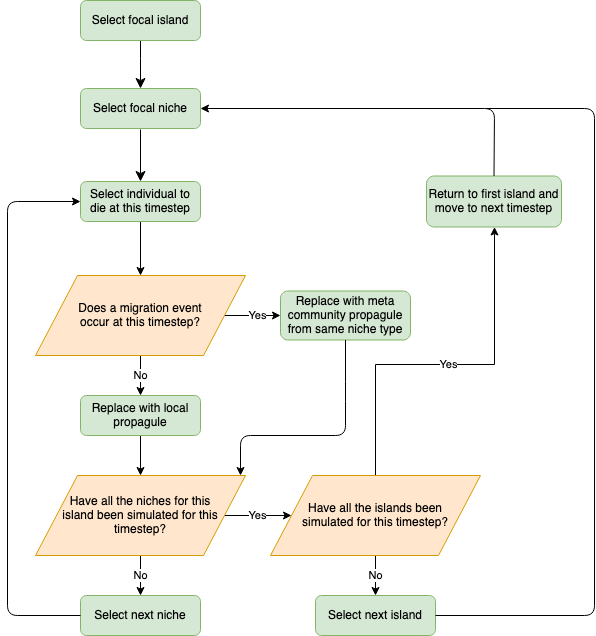
\includegraphics[scale=0.4]{../../Other/neutral_flowchart2.png}
  \caption{Flowchart of simulation design}
  \label{fig:Flowchart}
\end{figure}


\subsubsection{High Performance Computing}
The metacommunity and simulation code are contained in \textit{ClusterSim.R}. \textit{ClusterSim.R} functions are sourced by \textit{ClusterCode.R} and given the input parameters: \textit{J\_meta} = 50000, \textit{nu} = 0.001, \textit{num\_m\_rates} = 20, \textit{max\_k\_num} = 20, \textit{max\_k\_size} = 20, \textit{wall\_time} = 1380, \textit{output\_file\_name} = output\_file\_name (where each simulation is given a unique file name "simulation\_timeseries\_\textit{i}". \textit{ClusterRun.sh} is used to run on the cluster, with a time limit of 24:00:00. \textit{wall\_time} is given as 1380 minutes (23 hours) within the function, to ensure all simulations are completed before the cluster run ends. 100 parallel simulation were run on the Imperial College London High Performance Computing service. This generated a total of 800000 islands, simulated for $>$ 30000 timesteps.   

\subsection{Data Preparation and Timeseries Plots}
The 100 simulation results were imported into \textit{DataPrep.R}. The data from each island was isolated and configured into a data frame with simulation number, migration rate, area, number of niches and number of species (\textit{SimModelFitData.csv}). A second data frame was generated for timeseries plotting, with simulation number, island number, migration rate, timestep and species richness timeseries for each island (\textit{SimTimeseriesPlotData.csv}).\bigskip

\noindent To ensure the simulation had run long enough for each island to reach dynamic equilibrium the species richness timeseries of simulations 25, 50 and 75 were plotted(\textit{TimeseriesPlot.R})(Figure 2).

\subsection{Analysis}\bigskip

\begin{verbatim}
chisholm_model <- function(area, theta, m0, K) {
  rho = 1
  K = K
  Js = area*rho
  J_stars = Js/K
  ms = m0/sqrt(area)
  gamma_stars = J_stars*ms/(1-ms)
  return(theta*(digamma(theta/K+gamma_stars*
  (digamma(gamma_stars+J_stars)-digamma(gamma_stars)))-digamma(theta/K)))
}
\end{verbatim}

\noindent An analysis script (\textit{Analysis.R}) imported the prepared data (\textit{SimModelFitData.csv}) for each island across all simulations (800000 islands). Model estimated species richnesses were generated by giving the island parameters (\textit{m0 = m*sqrt(area)}) and an estimated \textit{theta} (\textit{theta = 2*(niche\_size*K)*nu}, where \textit{niche\_size * K} = size of each niche in the metacommunity from which immigration events can occur times by the number of niches contributing to the island community i.e. number of niches on the island). The results of the simulation and those estimated by the \textit{chisholm\_function} (above) were bound together in a data frame. Mean species richness results for each combination of island area, migration rate and number of niches across all 100 simulations was calculated and stored.


\section{Data Collection and Analysis}

\subsection{Datasets}

\begin{table}[h!]
  \begin{center}
    \caption{Summary of datasets collected from the literature}
    \label{table1}
    \pgfplotstabletypeset[
      multicolumn names, % allows to have multicolumn names
      col sep=comma, % the seperator in our .csv file
      display columns/0/.style={
		column name=$Attribute$, % name of first column
		string type},  % use siunitx for formatting
      display columns/1/.style={
		column name=$Aqua$,
		column type={S},string type},
      display columns/2/.style={
		column name=$Terra$,
		column type={S},string type},
      display columns/3/.style={
		column name=$Total$,
		column type={S},string type},
      every head row/.style={
		before row={\toprule}, % have a rule at top
		after row={
			%\si{\ampere} & \si{\volt}\\ % the units seperated by &
			\midrule} % rule under units
			},
		every last row/.style={after row=\bottomrule}, % rule at bottom
    ]{summary_stats.csv} % filename/path to file
  \end{center}
\end{table}

In-lieu of being able to generate my own dataset, I compiled 36 datasets of microbial species/taxa-area relationships. A full description of each dataset and their authors can be found in the Supplementary Material section. These datasets included a range of taxonomic groups, including archaea, bacteria, fungi, algae, protazoa and pathogens. The datasets also included aquatic and terrestrial habitats, as well as in-situ and lab based investigations. For the majority of datasets, the number of observed species, strains, operational taxonomic units or phylogroups per "island" habitat was taken. Some studies only supplied diversity indexes (gamma diversity, phylogenetic diversity, faiths dp, simpsons index, chao 1, T-RFLP, viral prevalence). The estimated number of cells/individuals per unit area was also taken from each study, or estimated from the relevant literature if unavailable.     

\subsection{Model Fitting}

\begin{equation}
S=\theta\{\psi(\frac{\theta}{K}+\gamma(\psi(\gamma+J)-\psi(\gamma)))-\psi(\frac{\theta}{K})\}
\end{equation} 

For each dataset I found initial parameter estimates for \textit{m} and $\theta$. I then looped through all values of \textit{K} from 1 to the maximum number of taxa recorded on one "island" and fitted the Chisholm model (2.1) using NLLS fitting. From the fitting, the best-fit parameters for \textit{m} and $\theta$ were selected, along with their best fit \textit{K}. On "islands" where the estimated cell count per unit area was less than the value of \textit{K}, estimated species richness was constrained to equal number of individuals so as not to more species than individual microorganisms. %%%is this neccessary???

Values for rho were either taken from the original paper or from the literature.

\subsection{Critical Area}

\begin{equation}
ACrit=\frac{\theta(1 - m)(exp(K/\theta) - 1}{m\rho*log(1/m)}
\end{equation}

For each successful model fitting, the critical area of transition from a niche-structured regime to an extinction-colonisation equilibrium regime was estimated. The best-fit values of \textit{K}, \textit{m} and $\theta$ from the model fitting were given to the critical area equation (2.2). By finding the critical area of regime transition for the datasets, I was able to test the theory that the regime shift would occur at lower areas for "islands" that are less isolated. I then conducted a multiple regression analysis with critical area as dependent variable and habitat type (aquatic/terrestrial) and taxonomic group as categorical variables. 

\chapter{Results}

%Results. Describe your results in a logical order: this may not necessarily be the order in which you did the experiments. Briefly summarise the main results at the end of each main experiment or sequence of associated experiments. Do not duplicate results -- put a table or a graph but not both unless the two methods of presentation demonstrate different points of importance. You must refer appropriately to figures or tables in the text and remember to emphasise and perhaps quote significant results. In particular, think about:

%o What were the results of your hypothesis tests, in the order you describe them in the Methods?
{\texorpdfstring
%TTo verify the fitting procedure for each of the three models (Classic, Depth, Perimeter) I created three different model simulations. I ran the simulation data through three NLLS fitting scripts to retrieve the known parameters ($\theta$, as calculated from \textit{nu} and metacommunity size \textit{J*K}, \textit{m\textsubscript{0}} and \textit{K}). Here I have plotted the know parameters against those estimated by the model fitting procedure. Once the model fitting procedures are validated, I use them to fit the three models to my datasets, as well as calculating critical area (\textit{A\textsubscript{crit}}) between niche-structured regime and colonisation-extinction regime. Using critical area estimates I test the hypothesis that regime change will occur at lower areas for more motile species and less isolated habitats. 

\section\section{Simulation}

\begin{figure}[htbp]
\centering
\subfloat[The Classic Model]{\label{fig:a}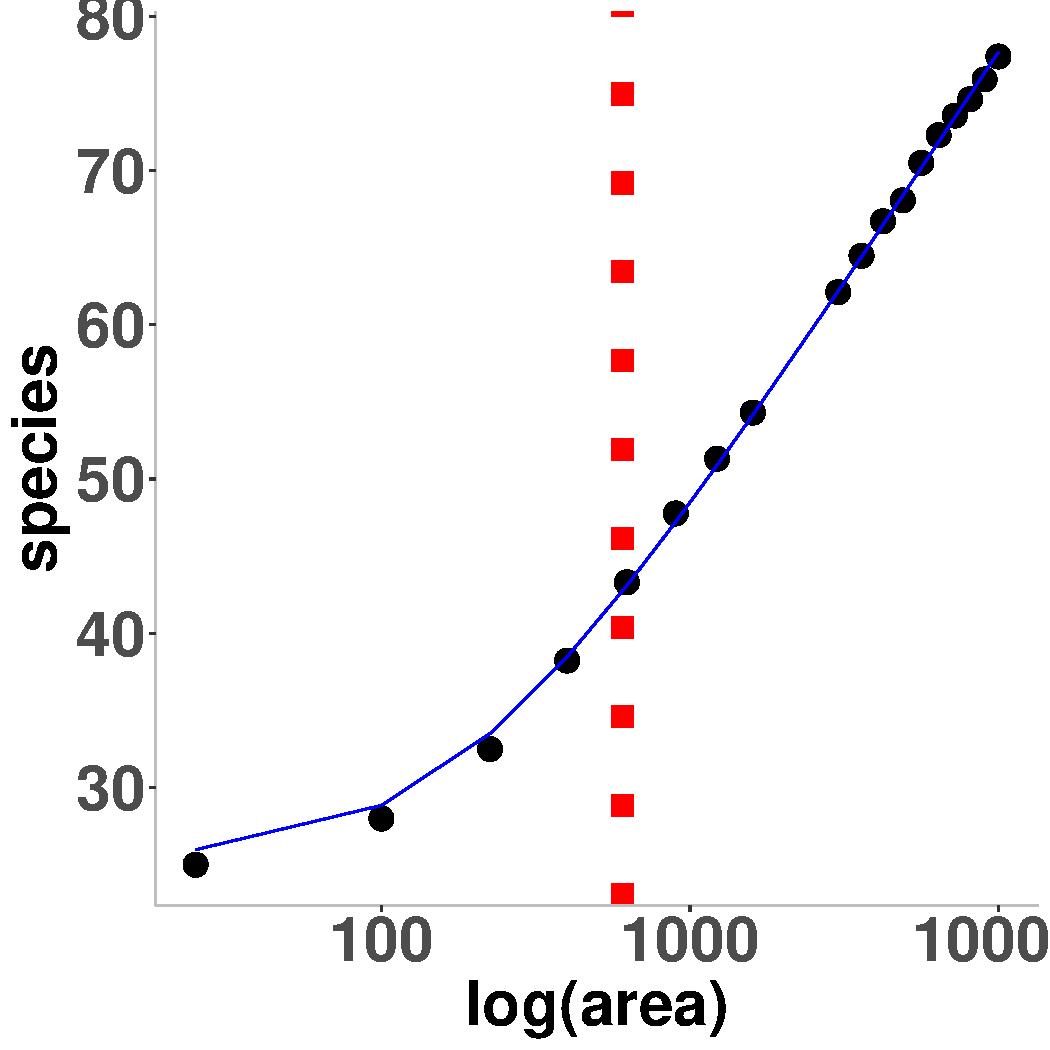
\includegraphics[width=0.3\linewidth]{../Results/Simulation/NLLSPlotClassic5.pdf}}
\subfloat[The Depth Model]{\label{fig:b}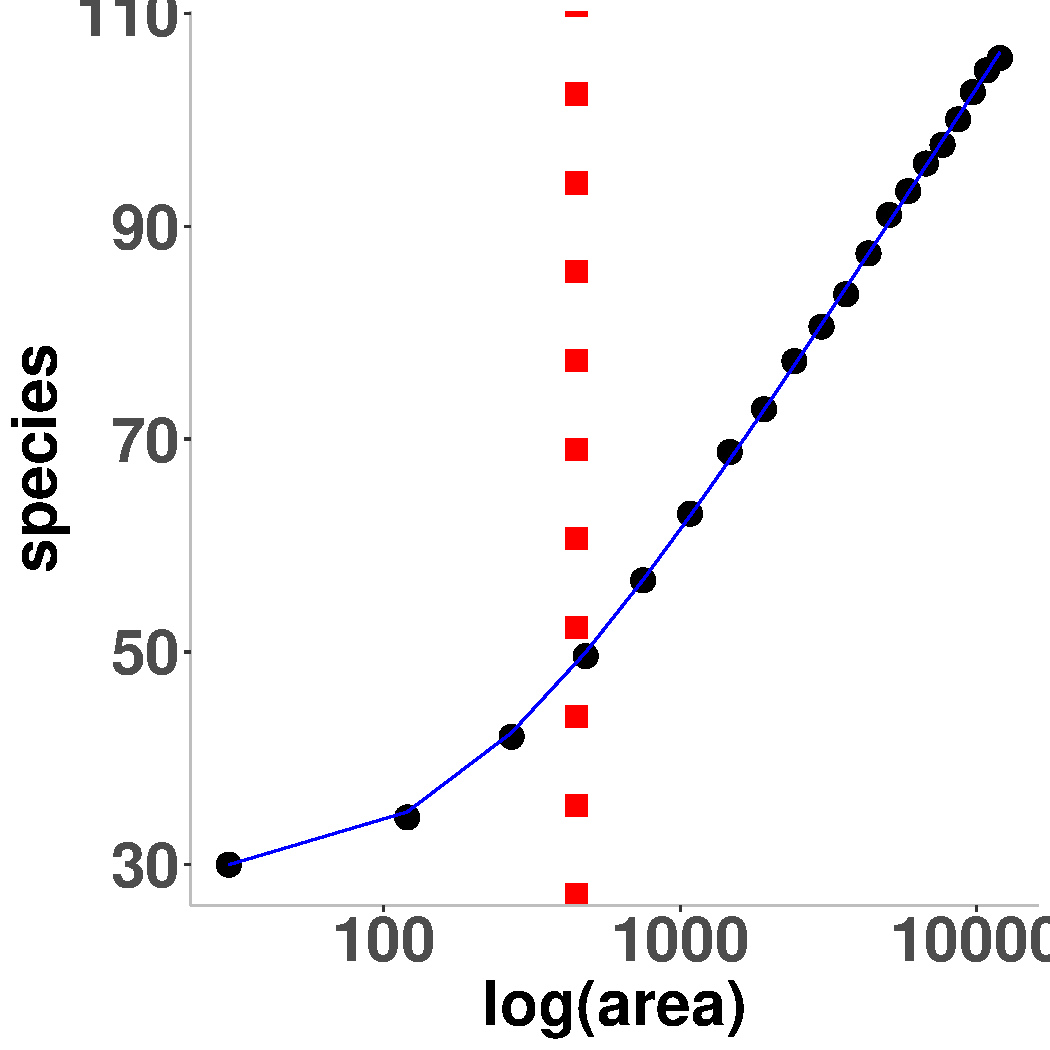
\includegraphics[width=0.3\linewidth]{../Results/Simulation/NLLSPlotDepth6.pdf}}
\subfloat[The Perimeter Model]{\label{fig:c}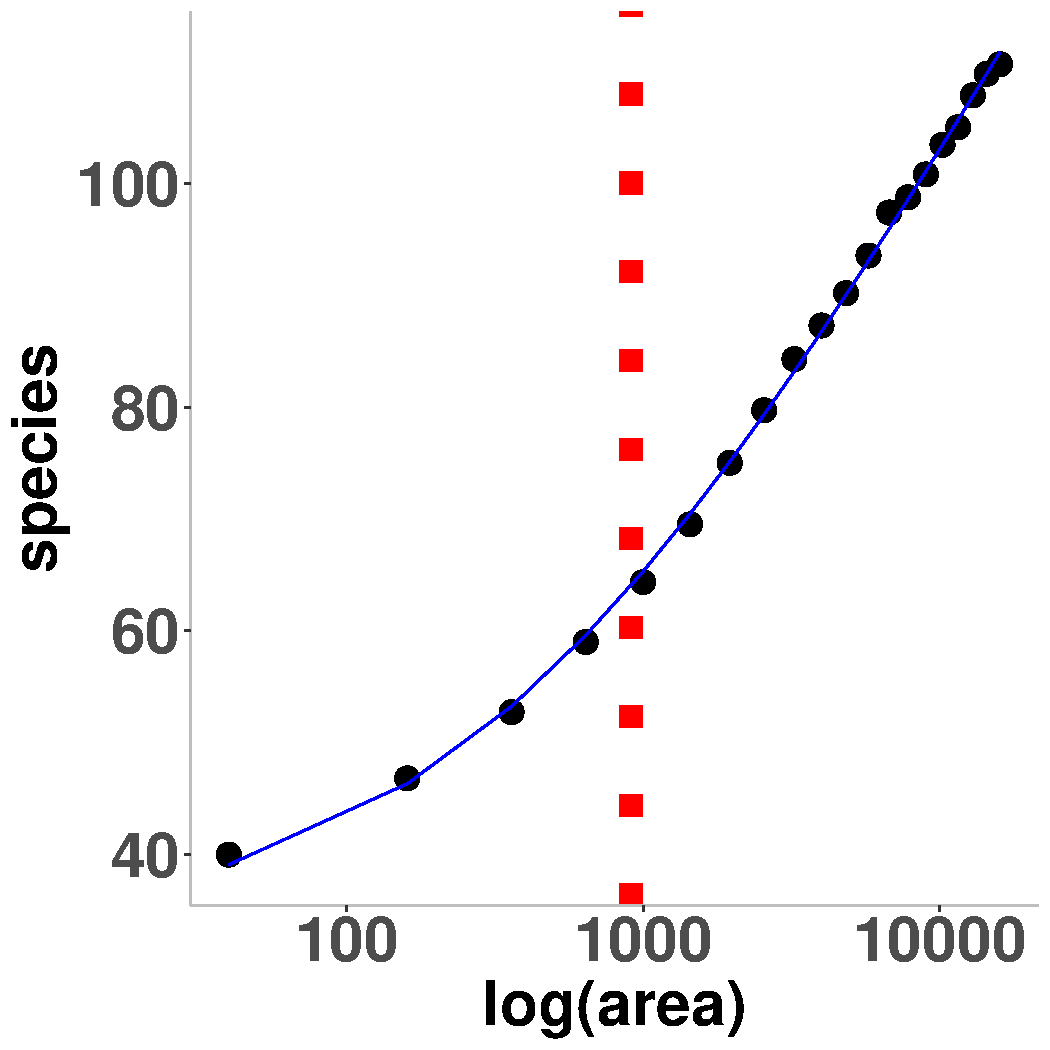
\includegraphics[width=0.3\textwidth]{../Results/Simulation/NLLSPlotPeri8.pdf}}
\bigskip 


Simulation data point \tikz\draw[black,fill=black] (0,0) circle (.5ex); \;\;NLLS fit \textcolor{blue}{\rule{1.5cm}{1mm}} \textit{A\textsubscript{crit}}\;\; \textcolor{red}{\rule{0.1cm}{1mm}}\; \textcolor{red}{\rule{0.1cm}{1mm}}\; \textcolor{red}{\rule{0.1cm}{1mm}}\; \textcolor{red}{\rule{0.1cm}{1mm}}\\

\caption{NLLS fitting of simulation data. A) The Classic Model with true parameters $\theta$=13, \textit{m\textsubscript{0}}=0.05, \textit{K}=25 and estimated parameters $\theta$=13, \textit{m\textsubscript{0}}=0.05, \textit{K}=25. B) The Depth Model with true parameters $\theta$=18, \textit{m\textsubscript{0}}=0.06, \textit{K}=30 and estimated parameters $\theta$=19, \textit{m\textsubscript{0}}=0.05, \textit{K}=30. C) The Perimeters Model with true parameters $\theta$=32, \textit{m\textsubscript{0}}=0.7, \textit{K}=40 and estimated parameters $\theta$=35, \textit{m\textsubscript{0}}=0.6, \textit{K}=39.}
\label{fig:myfig}
\end{figure}

\noindent My results verified that the simulation and analytic formula are in agreement as expected. The three \textit{A\textsubscript{crit}} formulas for each of the three model variations give reasonable estimations.

\subsection{Classic Model}

\noindent The Classic Model fitted the simulated data well. Estimated parameters were slightly higher than the true parameters for $\theta$ and slightly lower for \textit{m\textsubscript{0}} and \textit{K}. There was a significant difference between the true and estimated parameters for $\theta$ (p=0.0009, 9 df) and \textit{m\textsubscript{0}} (p=0.0002, 9 df). There was no significant difference in parameters for \textit{K} (p=0.08, 9 df).  As \textit{K} parameters showed no significant difference, and there was only a small difference between \textit{m\textsubscript{0}} and $\theta$ parameters, the model fitting process is considered validated and fit for applying to empirical datasets.   \\

\begin{figure}[htbp]
\centering
\subfloat[$\theta$ values]{\label{fig:a}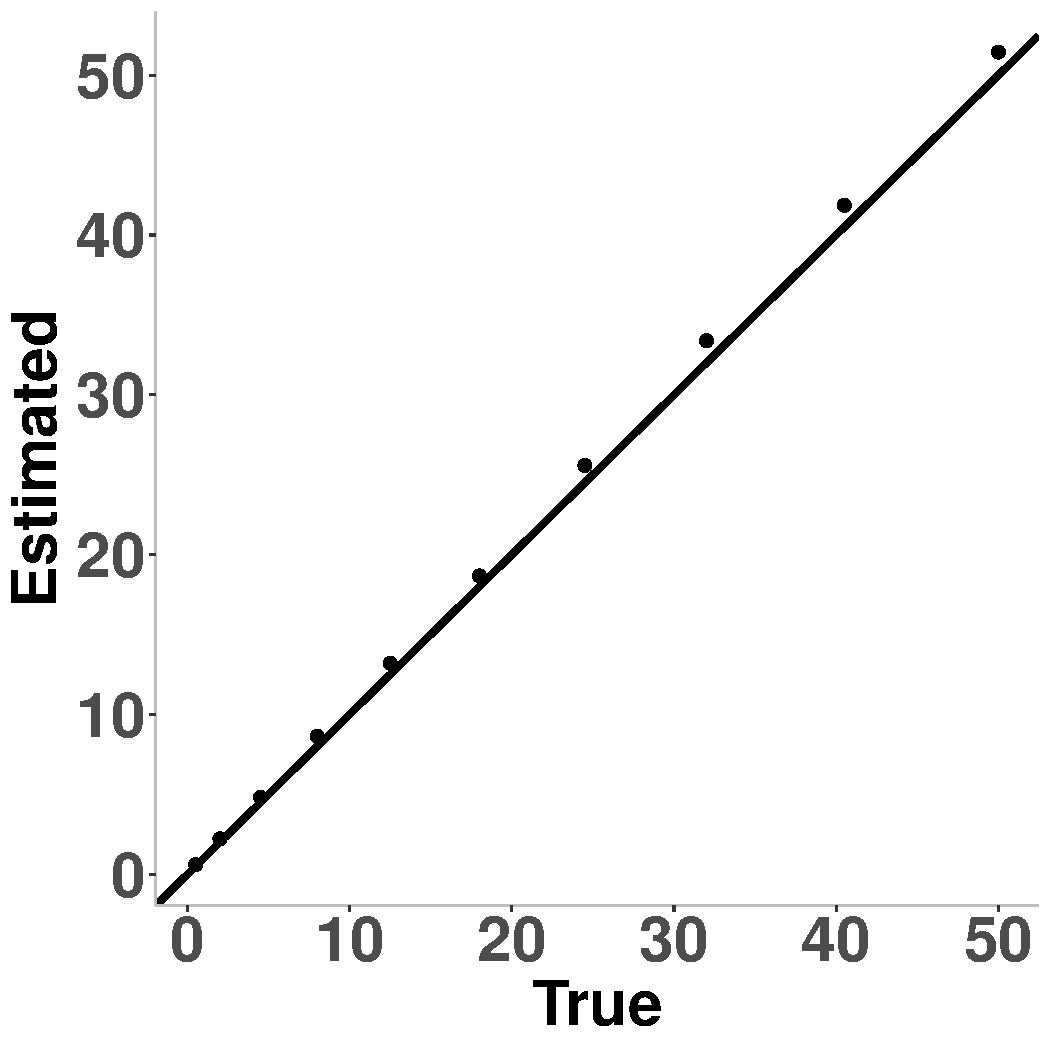
\includegraphics[width=0.3\linewidth]{AreaThetaResults.pdf}}
\subfloat[\textit{m\textsubscript{0}} values]{\label{fig:b}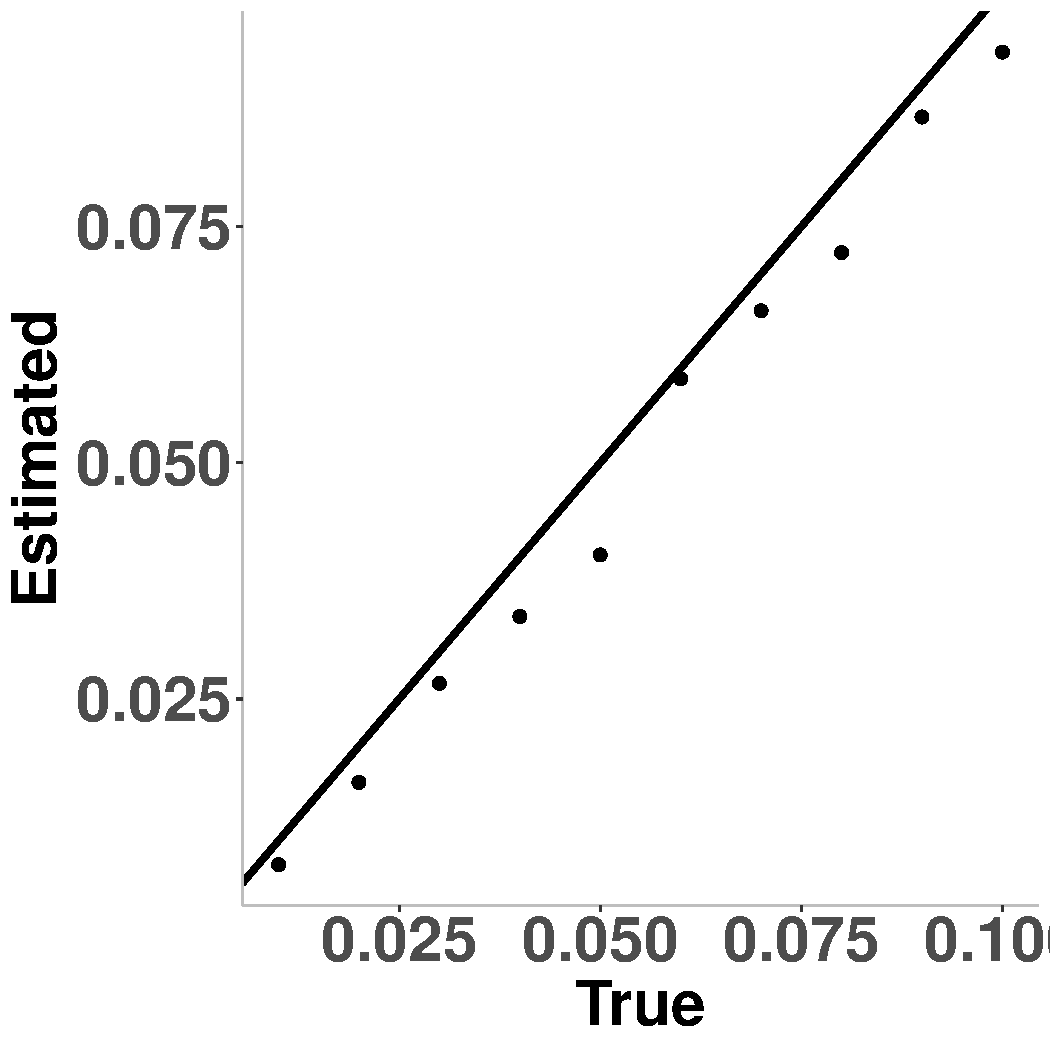
\includegraphics[width=0.3\linewidth]{Aream0Results.pdf}}
\subfloat[\textit{K} values]{\label{fig:c}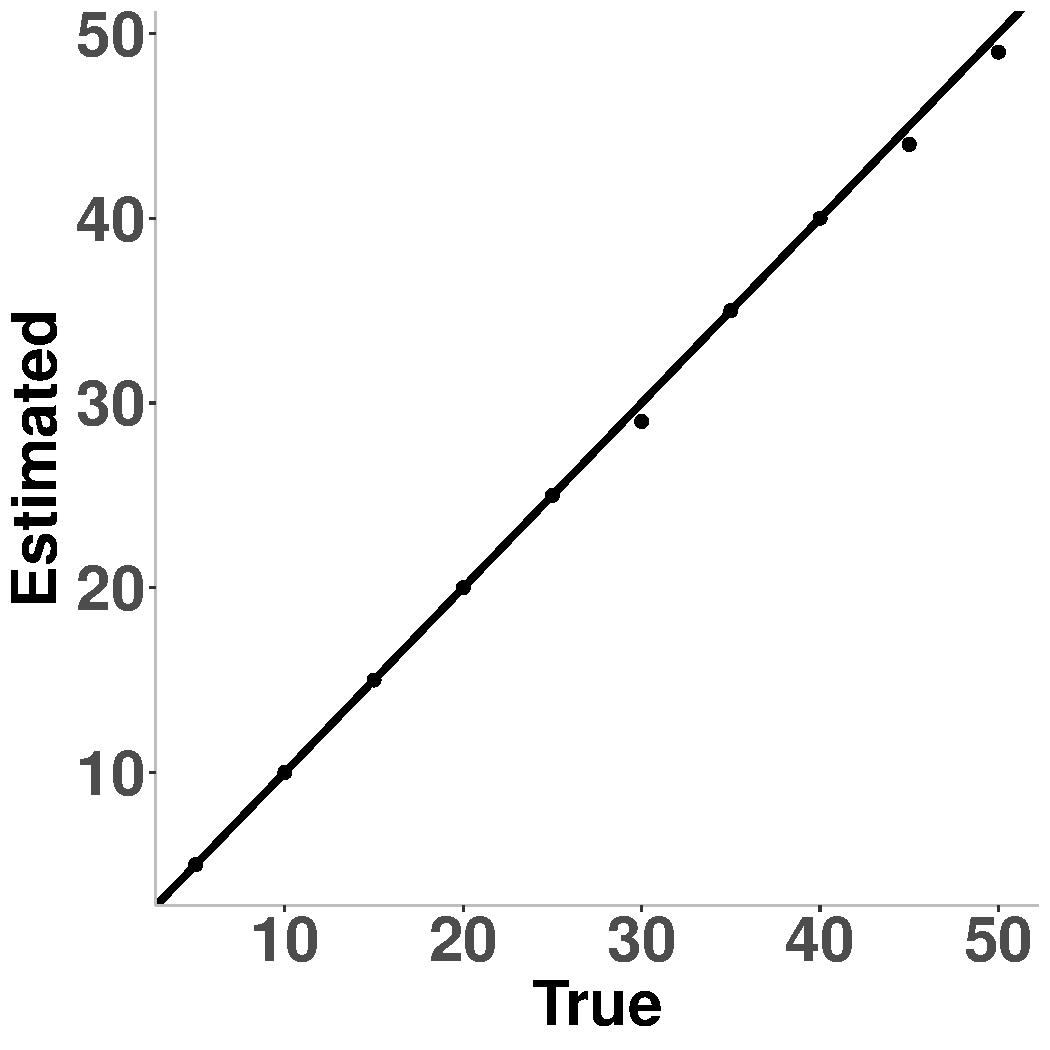
\includegraphics[width=0.3\textwidth]{AreaKResults.pdf}}
\bigskip

Parameter differences data point \tikz\draw[black,fill=black] (0,0) circle (.5ex); \;\; 1:1 line \textcolor{black}{\rule{1.5cm}{1mm}}\\

\caption{The true parameters values of $\theta$ (A), \textit{m\textsubscript{0}} (B) and \textit{K} (C) were simulated and the results fitted using the Classic Model analytical NLLS fitting procedure to get the parameters back. True and estimated values for the three fitted parameters are plotted above. Fittings of the Classic Model to simulated data returned mean R\textsuperscript{2} = 0.99, adjusted R\textsuperscript{2} = 0.99.}
\label{fig:myfig}
\end{figure}

\begin{table}[h!]
  \begin{center}
    \caption{Comparison between true and estimated mean parameters across 200 Classic Model simulations clustered into 10 groups where parameter values ($\theta$, \textit{m\textsubscript{0}}, \textit{K}) were the same for each simulation group with varying areas.}
    \label{table5}
    \pgfplotstabletypeset[
      multicolumn names, % allows to have multicolumn names
      col sep=comma, % the seperator in our .csv file
      display columns/0/.style={
		column name=$Parameter$, % name of first column
		string type},  % use siunitx for formatting
      display columns/1/.style={
		column name=$True$,
		column type={S},string type},
      display columns/2/.style={
		column name=$Estimated$,
		column type={S},string type},
      display columns/3/.style={
		column name=$Difference$,
		column type={S},string type},
           every head row/.style={
		before row={\toprule}, % have a rule at top
		after row={
			%\si{\ampere} & \si{\volt}\\ % the units seperated by &
			\midrule} % rule under units
			},
		every last row/.style={after row=\bottomrule}, % rule at bottom
    ]{ClassicParam.csv} % filename/path to file
  \end{center}
\end{table}



\subsection{Depth Model}

\noindent The Depth Model fitted the simulated data well. Estimated values of $\theta$ were higher, \textit{K} and \textit{m\textsubscript{0}} values were lower than the true parameters (Table 3.2). There was a significant difference between the true and estimated values for $\theta$ (p=0.0005, 9 df) and \textit{m\textsubscript{0}} (p=0.005, 9 df), but there was no significant difference for \textit{K} (p=0.168, 9 df). As \textit{K} showed no significant difference, and the difference in estimated $\theta$ and \textit{m\textsubscript{0}} values were low, the model fitting process is considered validated and fit for applying to empirical datasets.  

\begin{figure}[htbp]
\centering
\subfloat[$\theta$ values]{\label{fig:a}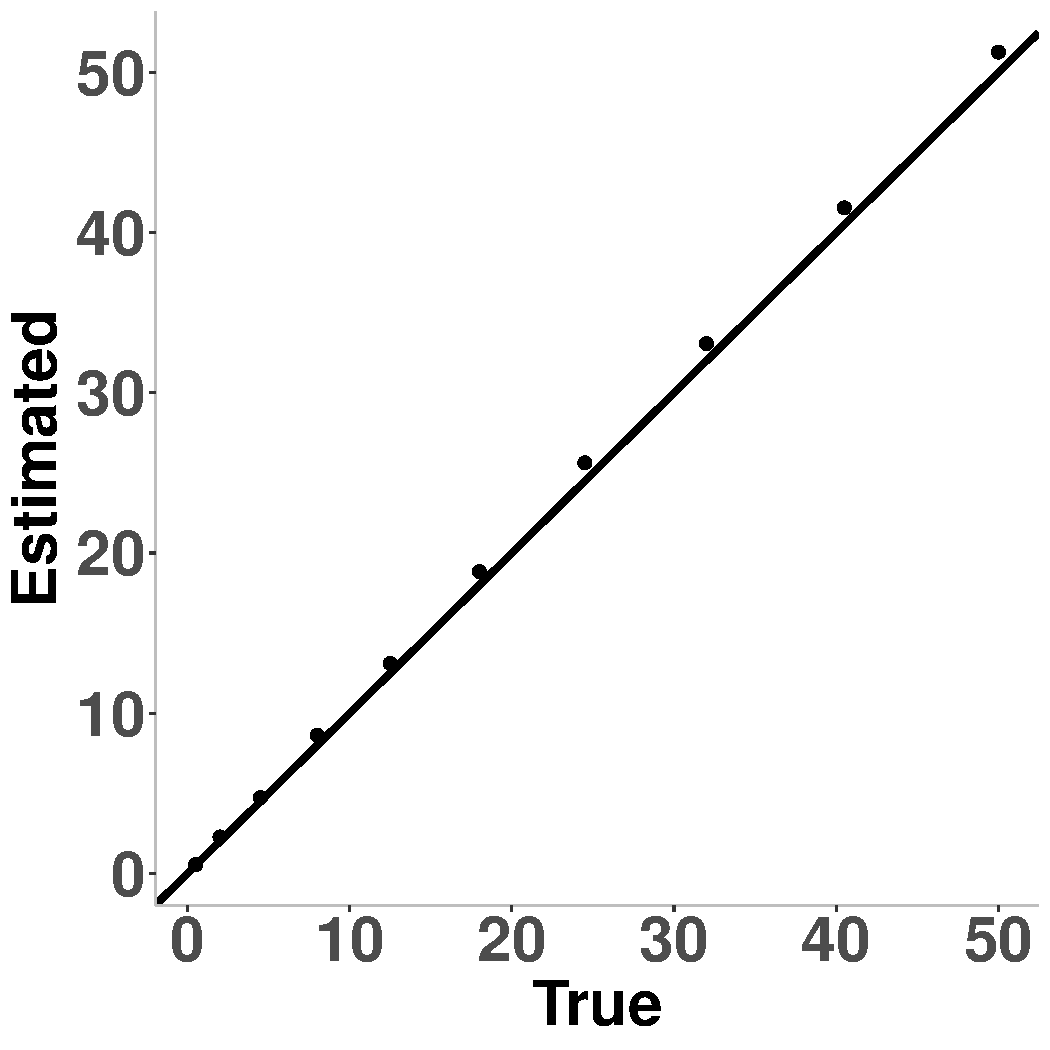
\includegraphics[width=0.3\linewidth]{DepthThetaResults.pdf}}
\subfloat[\textit{m\textsubscript{0}} values]{\label{fig:b}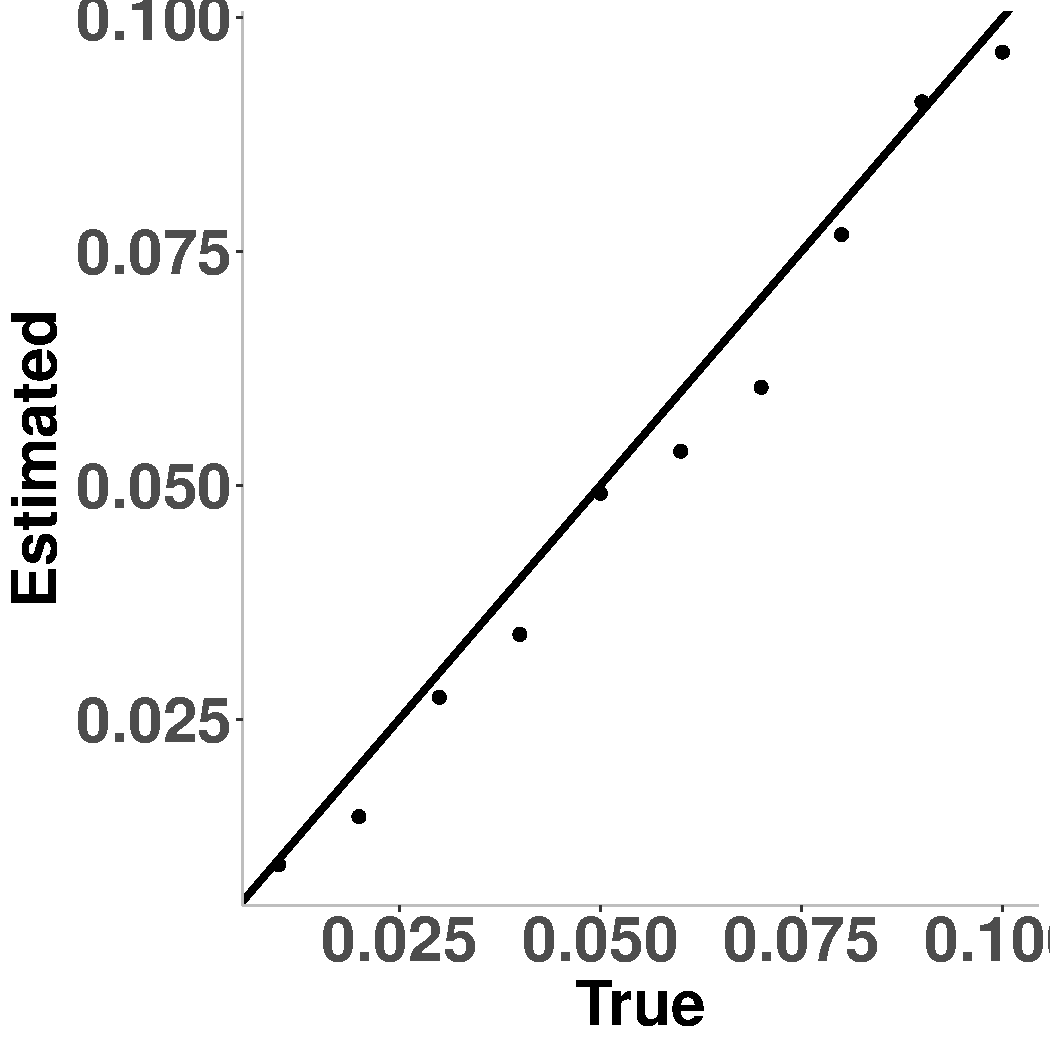
\includegraphics[width=0.3\linewidth]{Depthm0Results.pdf}}
\subfloat[\textit{K} values]{\label{fig:c}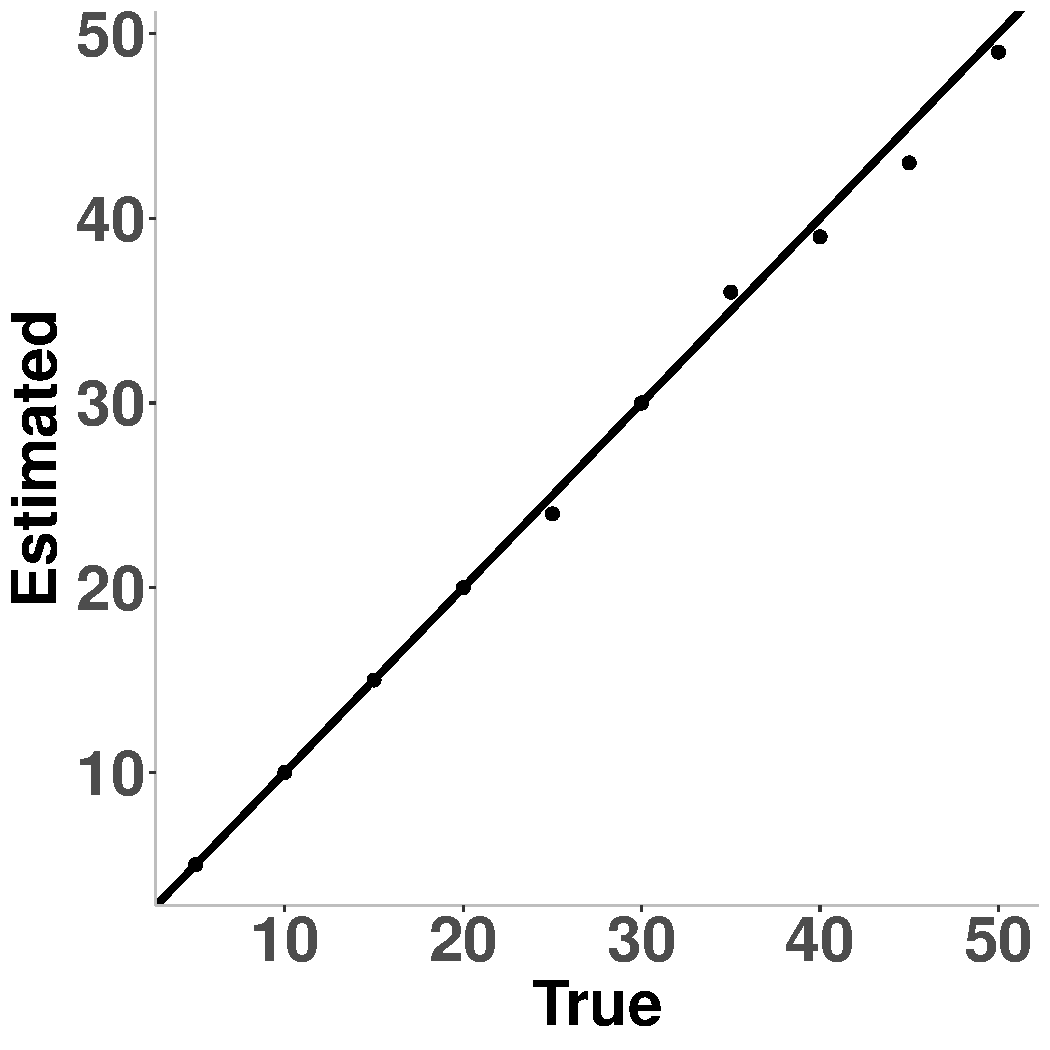
\includegraphics[width=0.3\textwidth]{DepthKResults.pdf}}
\bigskip

Parameter differences data point \tikz\draw[black,fill=black] (0,0) circle (.5ex); \;\; 1:1 line \textcolor{black}{\rule{1.5cm}{1mm}}\\

\caption{The true parameters values of $\theta$ (A), \textit{m\textsubscript{0}} (B) and \textit{K} (C) were simulated and the results fitted using the Depth Model analytical NLLS fitting procedure to get the parameters back. True and estimated values for the three fitted parameters are plotted above. Fittings of the Depth Model to simulated data returned mean R\textsuperscript{2} = 0.99, adjusted R\textsuperscript{2} = 0.99.}
\label{fig:myfig}
\end{figure}

\begin{table}[h!]
  \begin{center}
    \caption{Comparison between true and estimated mean parameters across 200 Depth Model simulations clustered into 10 groups where parameter values ($\theta$, \textit{m\textsubscript{0}}, \textit{K}) were the same for each simulation group with varying areas.}
    \label{table5}
    \pgfplotstabletypeset[
      multicolumn names, % allows to have multicolumn names
      col sep=comma, % the seperator in our .csv file
      display columns/0/.style={
		column name=$Parameter$, % name of first column
		string type},  % use siunitx for formatting
      display columns/1/.style={
		column name=$True$,
		column type={S},string type},
      display columns/2/.style={
		column name=$Estimated$,
		column type={S},string type},
      display columns/3/.style={
		column name=$Difference$,
		column type={S},string type},
           every head row/.style={
		before row={\toprule}, % have a rule at top
		after row={
			%\si{\ampere} & \si{\volt}\\ % the units seperated by &
			\midrule} % rule under units
			},
		every last row/.style={after row=\bottomrule}, % rule at bottom
    ]{DepthParam.csv} % filename/path to file
  \end{center}
\end{table} 


\subsection{Perimeter Model}


\begin{figure}[htbp]
\centering
\subfloat[$\theta$ values]{\label{fig:a}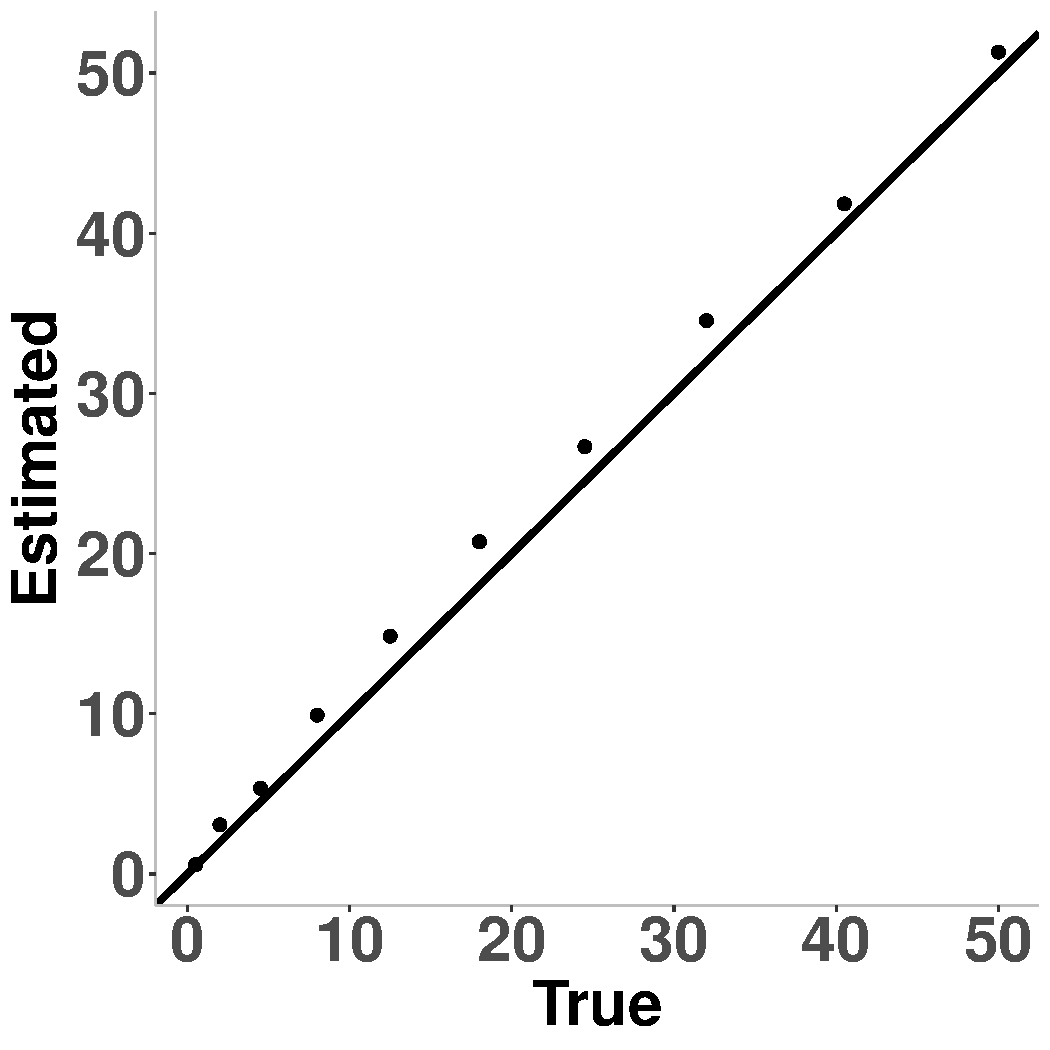
\includegraphics[width=0.3\linewidth]{PeriThetaResults.pdf}}
\subfloat[\textit{m\textsubscript{0}} values]{\label{fig:b}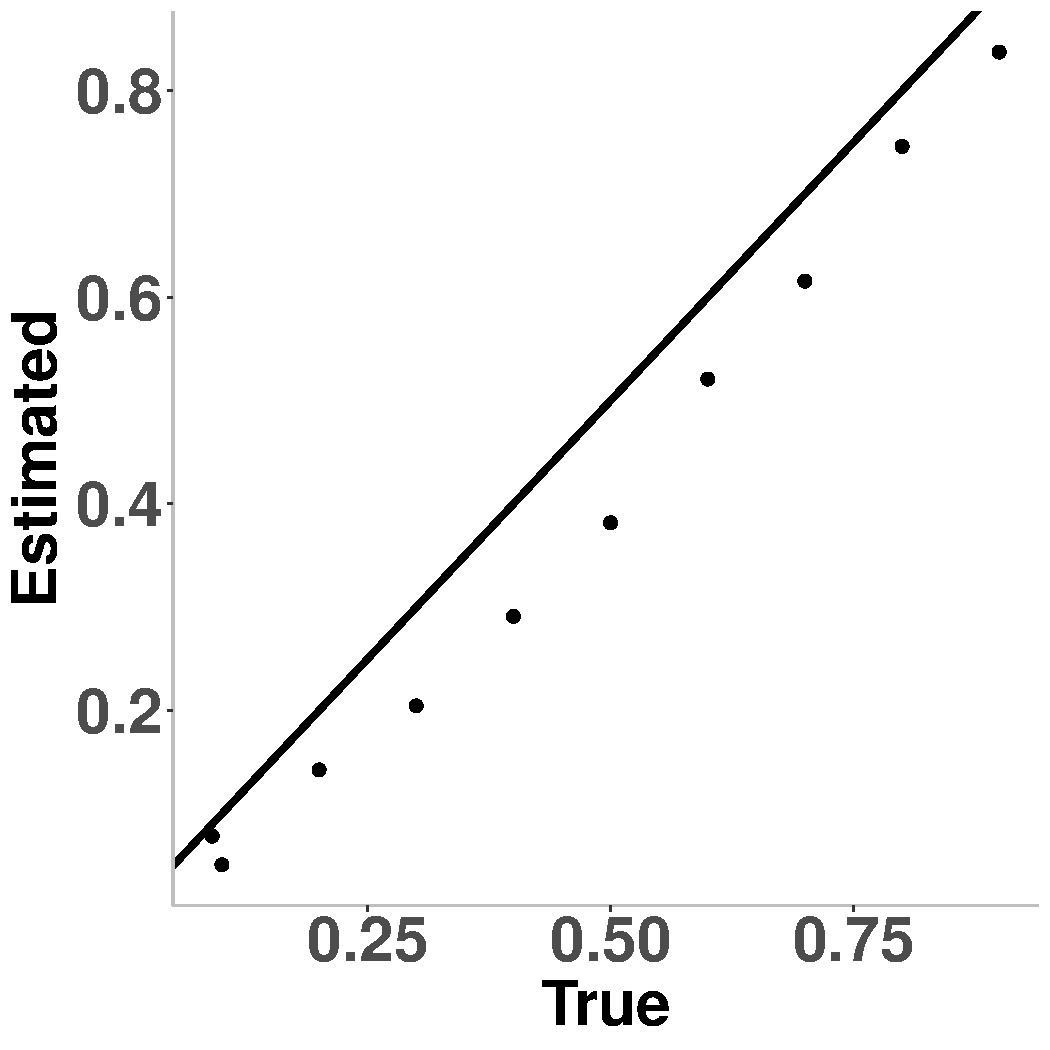
\includegraphics[width=0.3\linewidth]{Perim0Results.pdf}}
\subfloat[\textit{K} values]{\label{fig:c}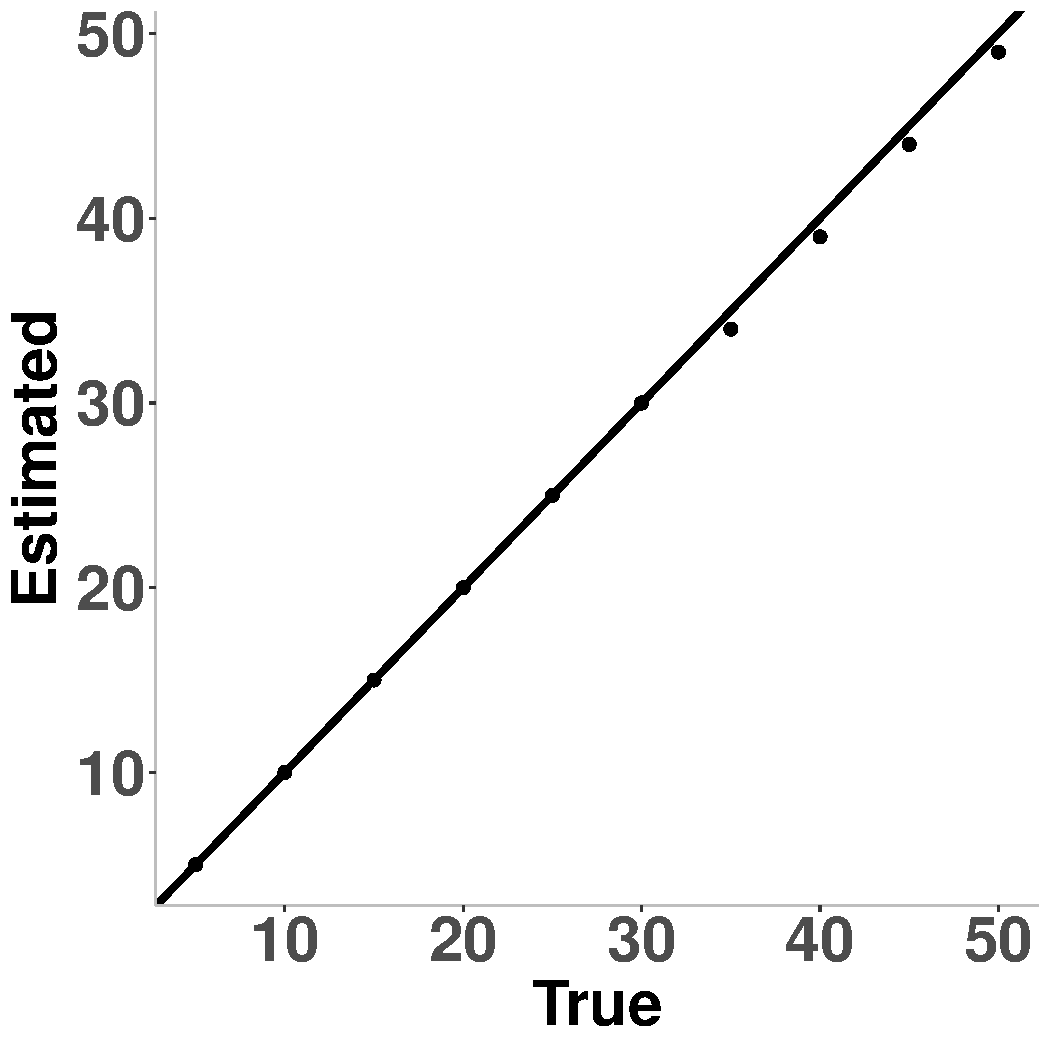
\includegraphics[width=0.3\textwidth]{PeriKResults.pdf}}
\bigskip

Parameter differences data point \tikz\draw[black,fill=black] (0,0) circle (.5ex); \;\; 1:1 line \textcolor{black}{\rule{1.5cm}{1mm}}\\

\caption{The true parameters values of $\theta$ (A), \textit{m\textsubscript{0}} (B) and \textit{K} (C) were simulated and the results fitted using the Perimeter Model analytical NLLS fitting procedure to get the parameters back. True and estimated values for the three fitted parameters are plotted above. Fittings of the Perimeter Model to simulated data returned mean R\textsuperscript{2} = 0.99, adjusted R\textsuperscript{2} = 0.99.}
\label{fig:myfig}
\end{figure}

\begin{table}[h!]
  \begin{center}
    \caption{Comparison between true and estimated mean parameters across 200 Perimeter Model simulations clustered into 10 groups where parameter values ($\theta$, \textit{m\textsubscript{0}}, \textit{K}) were the same for each simulation group with varying areas.}
    \label{table5}
    \pgfplotstabletypeset[
      multicolumn names, % allows to have multicolumn names
      col sep=comma, % the seperator in our .csv file
      display columns/0/.style={
		column name=$Parameter$, % name of first column
		string type},  % use siunitx for formatting
      display columns/1/.style={
		column name=$True$,
		column type={S},string type},
      display columns/2/.style={
		column name=$Estimated$,
		column type={S},string type},
      display columns/3/.style={
		column name=$Difference$,
		column type={S},string type},
           every head row/.style={
		before row={\toprule}, % have a rule at top
		after row={
			%\si{\ampere} & \si{\volt}\\ % the units seperated by &
			\midrule} % rule under units
			},
		every last row/.style={after row=\bottomrule}, % rule at bottom
    ]{PeriParam.csv} % filename/path to file
  \end{center}
\end{table}

\noindent The Perimeter Model fitted the simulated data well. Estimated parameters for $\theta$ were slightly higher than true parameters, whilst \textit{m\textsubscript{0}} and \textit{K} were slightly lower than the true parameters (Table 3.3). There was significant difference between the true and estimated values for $\theta$ (p=0.0002, 9 df), \textit{m\textsubscript{0}} (p=5x10\textsuperscript{5}, 9 df) and \textit{K} (p=0.04, 9df). Despite the significant difference between the estimated and true values, the differences are small and the model fitting process is considered validated and fit for applying to empirical datasets.   

\section{Model Fitting}

\subsection{Non-Linear Least Squares Fitting}


\noindent 50 of the 57 datasets exhibited a positive TAR and were used for the NLLS fitting. Of the 50 datasets 26 failed to achieve adjusted R\textsuperscript{2} scores of between 0 and 1. These datasets were excluded from further analysis (see Supplementary Materials, Figure 7.2). 

\begin{table}[h!]
  \begin{center}
    \caption{The mean R\textsuperscript{2} and adjusted R\textsuperscript{2} results for each model (Classic, Depth, Perimeter) after being successfully fitted to 24 empirical datasets.}
    \label{table5}
    \pgfplotstabletypeset[
      multicolumn names, % allows to have multicolumn names
      col sep=comma, % the seperator in our .csv file
      display columns/0/.style={
		column name=$Model$, % name of first column
		string type},  % use siunitx for formatting
      display columns/1/.style={
		column name=$R\textsuperscript{2}$,
		column type={S},string type},
      display columns/2/.style={
		column name=$Adj R\textsuperscript{2}$,
		column type={S},string type},
           every head row/.style={
		before row={\toprule}, % have a rule at top
		after row={
			%\si{\ampere} & \si{\volt}\\ % the units seperated by &
			\midrule} % rule under units
			},
		every last row/.style={after row=\bottomrule}, % rule at bottom
    ]{RResults.csv} % filename/path to file
  \end{center}
\end{table}

\noindent All three models had similar mean R\textsuperscript{2} and adjusted R\textsuperscript{2} scores and fit the data moderately well (Table 3.4). The Classic Model was best-fit for 1 dataset, Depth and Perimeter were best for 2 each and the rest of the datasets were either best described by both Classic and Depth or all of the models (Table 3.5).  \\

\begin{table}[h!]
  \begin{center}
    \caption{The best-fit models (Classic, Depth, Perimeter) by highest adjusted R\textsuperscript{2} value for each empirical dataset (note some datasets had equal adjusted R\textsuperscript{2} values for two or more models). }
    \label{table5}
    \pgfplotstabletypeset[
      multicolumn names, % allows to have multicolumn names
      col sep=comma, % the seperator in our .csv file
      display columns/0/.style={
		column name=$Models$, % name of first column
		string type},  % use siunitx for formatting
      display columns/1/.style={
		column name=$Best Fit$,
		column type={S},string type},
           every head row/.style={
		before row={\toprule}, % have a rule at top
		after row={
			%\si{\ampere} & \si{\volt}\\ % the units seperated by &
			\midrule} % rule under units
			},
		every last row/.style={after row=\bottomrule}, % rule at bottom
    ]{BestModel.csv} % filename/path to file
  \end{center}
\end{table}

\noindent The best model fits had mean R\textsuperscript{2} = 0.49 and mean adjusted R\textsuperscript{2} = 0.41 with standard deviation 0.28 and range 0.01 - 0.96. The median value of $\theta$ was 8, with a range of 0.28 -- 159709. The median value of \textit{m\textsubscript{0}} was 2.17 x10\textsuperscript{-9} with a range of 4.97 x 10\textsuperscript{-16} -- 0.56. The median value for \textit{K} was 7, with range 1 -- 424. There was no correlation between the best fitted-values of the four parameters (Table 3.6). \\

\begin{table}[h!]
  \begin{center}
    \caption{p-values of correlations between the four model parameters ($\theta$, \textit{m\textsubscript{0}}, \textit{K}, $\rho$) that show no correlation}
    \label{table5}
    \pgfplotstabletypeset[
      multicolumn names, % allows to have multicolumn names
      col sep=comma, % the seperator in our .csv file
      display columns/0/.style={
		column name=$Parameter$, % name of first column
		string type},  % use siunitx for formatting
      display columns/1/.style={
		column name=$K$,
		column type={S},string type},
      display columns/2/.style={
		column name=$Theta$,
		column type={S},string type},
        display columns/3/.style={
		column name=$m\textsubscript{0}$,
		column type={S},string type},
	 display columns/4/.style={
		column name=$rho$,
		column type={S},string type},
           every head row/.style={
		before row={\toprule}, % have a rule at top
		after row={
			%\si{\ampere} & \si{\volt}\\ % the units seperated by &
			\midrule} % rule under units
			},
		every last row/.style={after row=\bottomrule}, % rule at bottom
    ]{Spearmansrank_p_corr.csv} % filename/path to file
  \end{center}
\end{table}

%How often was the power-law model a better fit to the data than the three models?
\noindent The power-law model had the same number of successful fittings as the Classic, Depth and Perimeter models. After removing failed fits the mean \textit{z} value was 0.16. The power-law model performed more poorly than the other three models (R\textsuperscript{2}=0.47, adjusted R\textsuperscript{2}=0.38) (see Supplementary Materials, Table 7.3). AIC scores indicated that the power-law model was not a more parsimonious model than the Classic, Depth or Perimeter models relative to model fit for any of the datasets (see Supplementary Materials, Table 7.4). The Classic and Depth models were significantly better than the power-law model for 9 datasets each. The Perimeter model was a better fit than the power-law model for 5 datasets.   
  
\section{Critical Area}
{\texorpdfstring
Off the five habitat types (terrestrial, riverine, lacustrine, plant and machine) and six taxonomic groups (algae, archaea, bacteria, fungi, pathogens and protozoa), the riverine habitat and archaea group did not have any successful fittings and are excluded from the following analysis.\\


\begin{figure}[htbp]
\centering
\subfloat[Dataset 45, bacteria in biomembrane reactors]{\label{fig:a}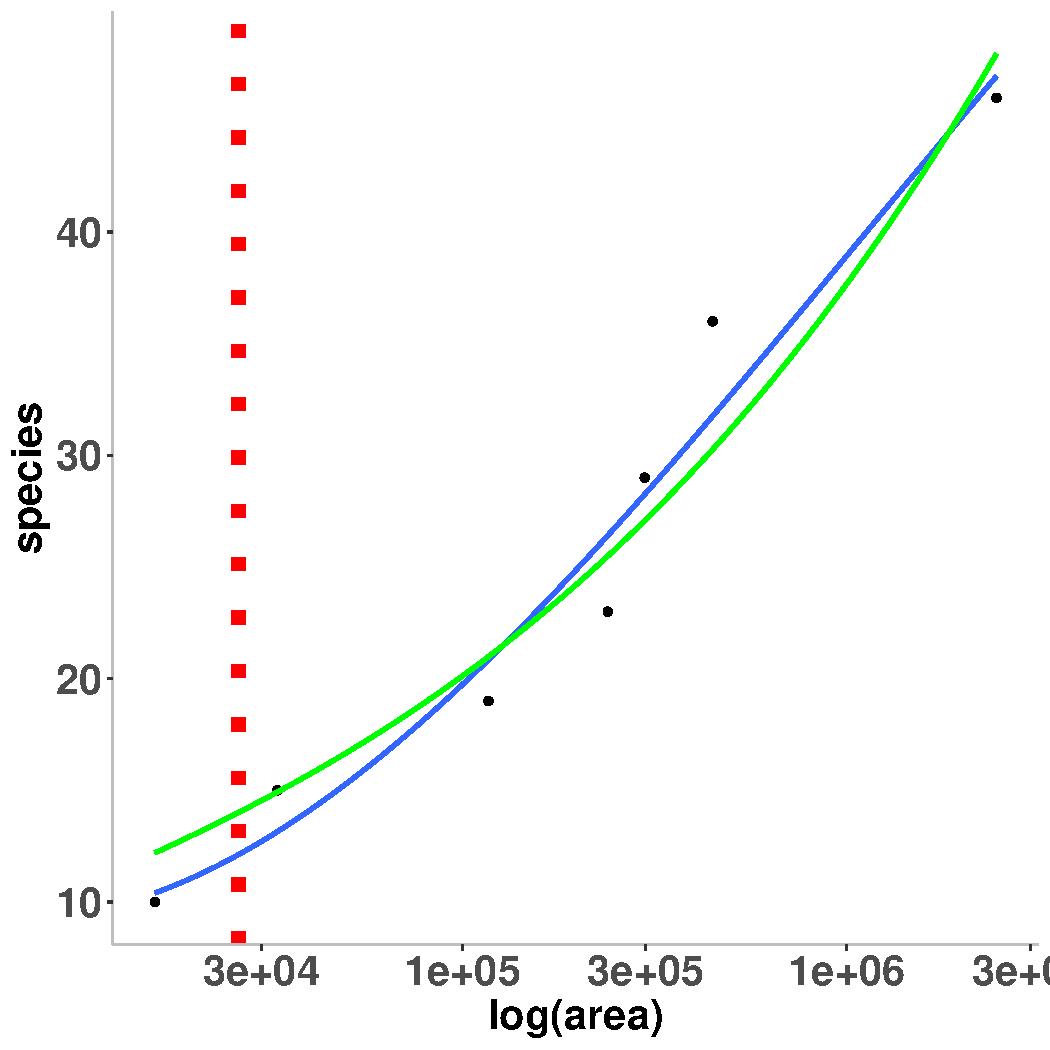
\includegraphics[width=0.45\linewidth]{../Results/ClassicNLLSPlot39.pdf}}\qquad
\subfloat[Dataset 44, fungi in plant root soil]{\label{fig:b}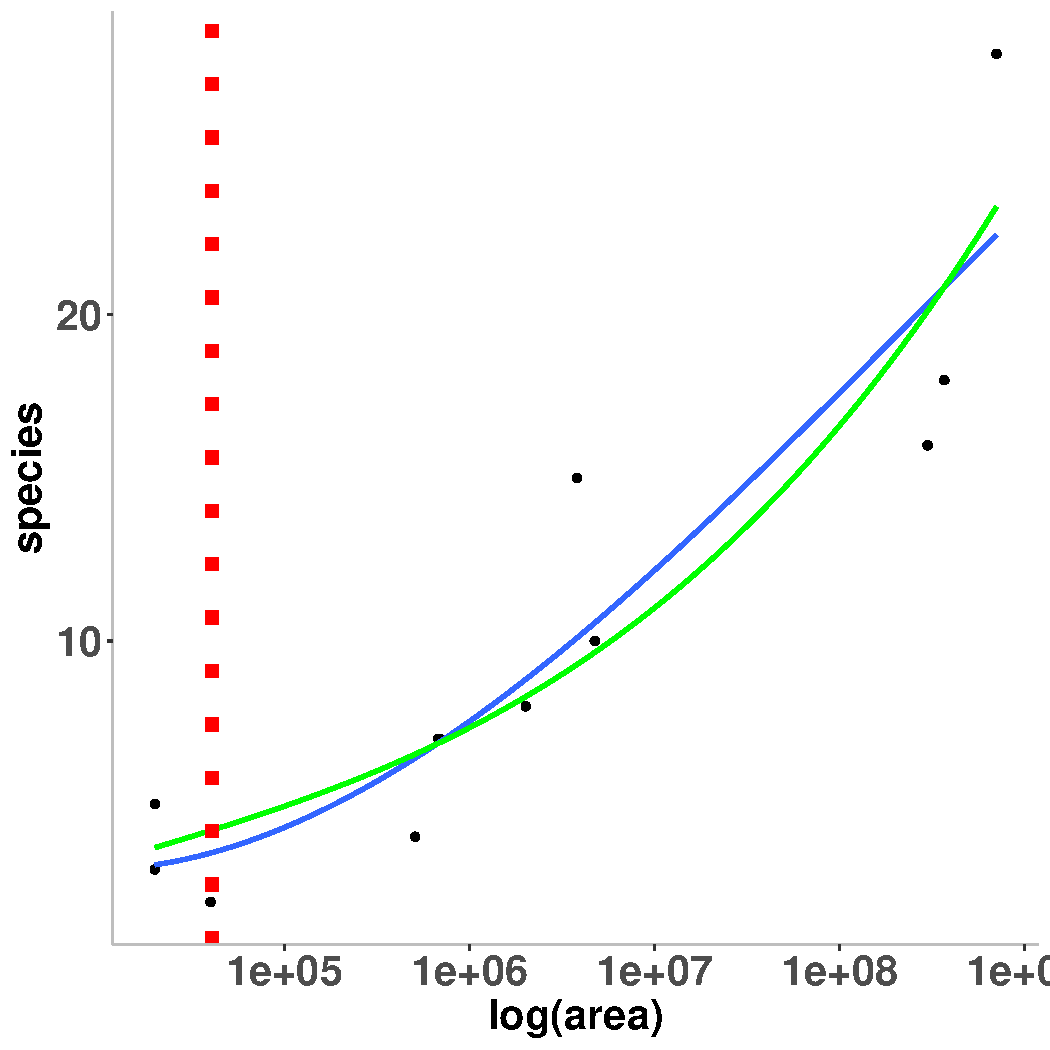
\includegraphics[width=0.45\linewidth]{../Results/PeriNLLSPlot38.pdf}}\\
\subfloat[Dataset 46, bacteria in tree holes (log area plotted with depth)]{\label{fig:c}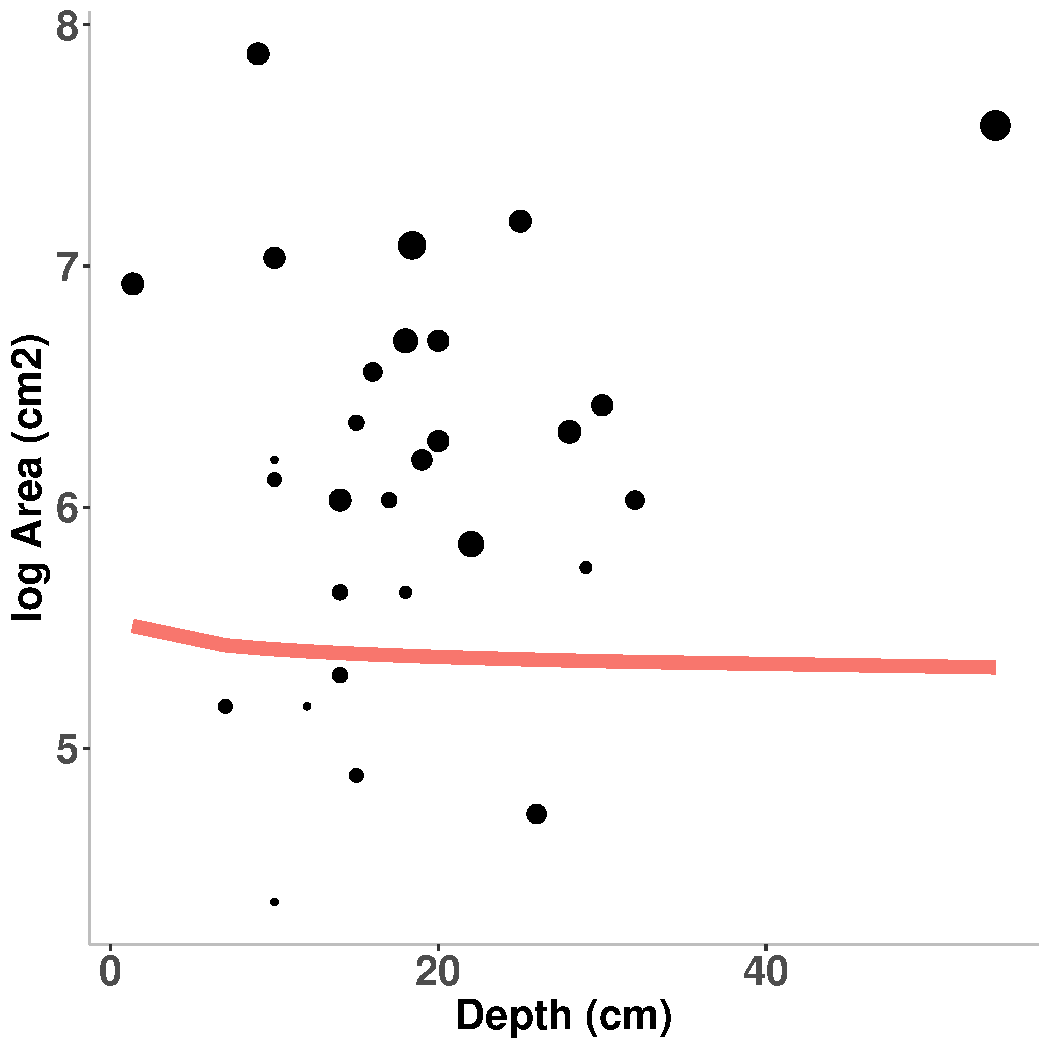
\includegraphics[width=0.45\textwidth]{../Results/DepthNLLSPlot40.pdf}}\qquad%
\subfloat[Dataset 46, bacteria in tree holes (log volume plotted with OTU richness)]{\label{fig:d}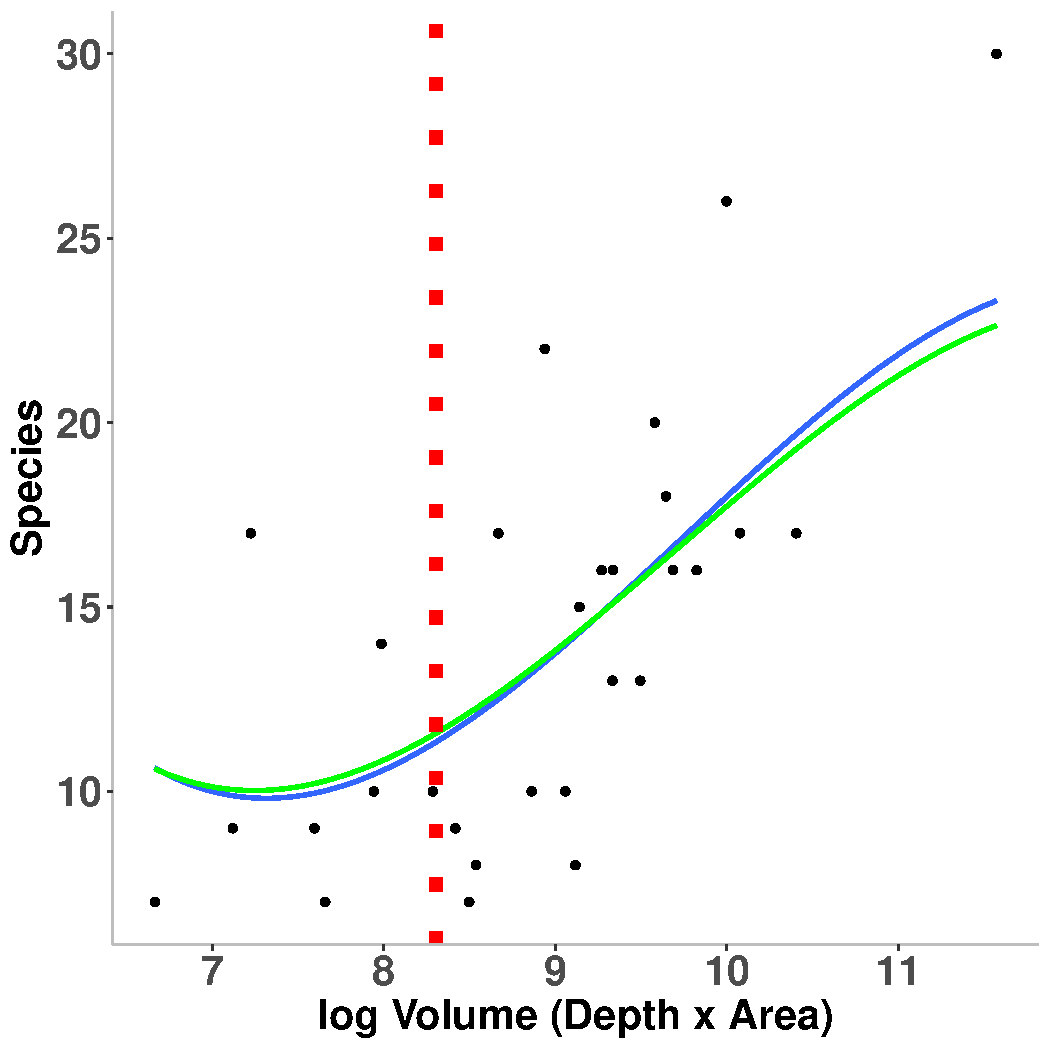
\includegraphics[width=0.45\textwidth]{../Results/DepthNLLSPlot2_40.pdf}}%
\bigskip

Simulation data point \tikz\draw[black,fill=black] (0,0) circle (.5ex); \;\;NLLS fit \textcolor{blue}{\rule{1.5cm}{1mm}} \;\;Power-Law fit \textcolor{green}{\rule{1.5cm}{1mm}}\;\; \textit{A\textsubscript{crit}/A\textsubscript{vol}}\;\; \textcolor{red}{\rule{0.1cm}{1mm}}\; \textcolor{red}{\rule{0.1cm}{1mm}}\; \textcolor{red}{\rule{0.1cm}{1mm}}\; \textcolor{red}{\rule{0.1cm}{1mm}}\\

\caption{A) Best-fit Classic Model for dataset 45, bacteria in biomembrane reactors. Red line indicates \textit{A\textsubscript{crit}}, blue line indicates NLLS fit and green line indicates power-law fit (NLLS fit: R\textsuperscript{2}=0.96, adjusted R\textsuperscript{2}=0.88, $\theta$=9, \textit{m\textsubscript{0}}=4.97 x 10\textsuperscript{-16}, \textit{K}=7, power-law fit: R\textsuperscript{2}=0.94, adjusted R\textsuperscript{2}=0.82, \textit{z}=0.27, \textit{c}=0.88). B) Best-fit Perimeter Model for dataset 44, fungi in plant soil (NLLS fit: R\textsuperscript{2}=0.85, adjusted R\textsuperscript{2}=0.77, $\theta$=5, \textit{m\textsubscript{0}}=6.15 x 10\textsuperscript{-11}, \textit{K}=2, power-law fit: R\textsuperscript{2}=0.87, adjusted R\textsuperscript{2}=0.78, \textit{z}=0.18, \textit{c}=0.64). C) Best-fit Depth Model for dataset 46, bacteria in freshwater treeholes. The size of the black circles represents increasing OTU richness at that corresponding depth (x-axis) and log area (y axis) (R\textsuperscript{2}=49, adjusted R\textsuperscript{2}=0.40, $\theta$=8, \textit{m\textsubscript{0}}=3.75 x 10\textsuperscript{-9}, \textit{K}=6, power-law fit: R\textsuperscript{2}=0.46, adjusted R\textsuperscript{2}=0.38, \textit{z}=0.33, \textit{c}=1.74). Where the red line passes through depth and area space is where \textit{A\textsubscript{crit}} occurs. D) Dataset 46 plotted as log Volume by OTU richness to illustrate the model fit and log critical volume (A\textsubscript{vol})}
\label{fig:myfig}
\end{figure}

\noindent The log \textit{A\textsubscript{crit}} data were not normally distributed with non-homogenous variances. Despite the violation of normality I have proceeded with the multiple regression analysis, although interpretation of results will take this into consideration. \\

\noindent Initial multiple regression revealed that the model was a poor fit to the data (R\textsuperscript{2}=0.39, adjusted R\textsuperscript{2}=0.05, p=0.374) and neither categorical variable was significant in predicting log \textit{A\textsubscript{crit}} (habitat type p=0.1759, taxonomic group p=0.6402). A plot of the model indicated that there was an outlying data point. After removing the outlying data point the model was significant in describing the data (R\textsuperscript{2}=0.62, adjusted R\textsuperscript{2}=0.44, p=0.02). Taxonomic group became weakly significant in predicting log \textit{A\textsubscript{crit}} (p=0.0187), habitat type did not (p=0.097). After removing habitat type as a variable the model was a similar fit to the data but more significant (R\textsuperscript{2}=0.55, adjusted R\textsuperscript{2}=0.45, p=0.004).\\

\noindent Multiple regression including taxonomic group upheld the prediction that \textit{A\textsubscript{crit}} would occur at lower areas for more motile OTUs as bacteria show the lowest log\textit{A\textsubscript{crit}} estimate and host-dependent pathogens show the highest (Table 3.7). \\

\noindent There was a large variation in mean log \textit{A\textsubscript{crit}} between habitats and taxonomic groups. Terrestrial habitats showed the highest mean log \textit{A\textsubscript{crit}} (27.33), whilst machine habitats showed the lowest (4.66) (Figure 3.6). Pathogens exhibited the largest mean log \textit{A\textsubscript{crit}} for taxonomic groups (55.15), with bacteria having the lowest (4.06) (Figure 3.6). \\

\begin{figure}[htp]

\centering
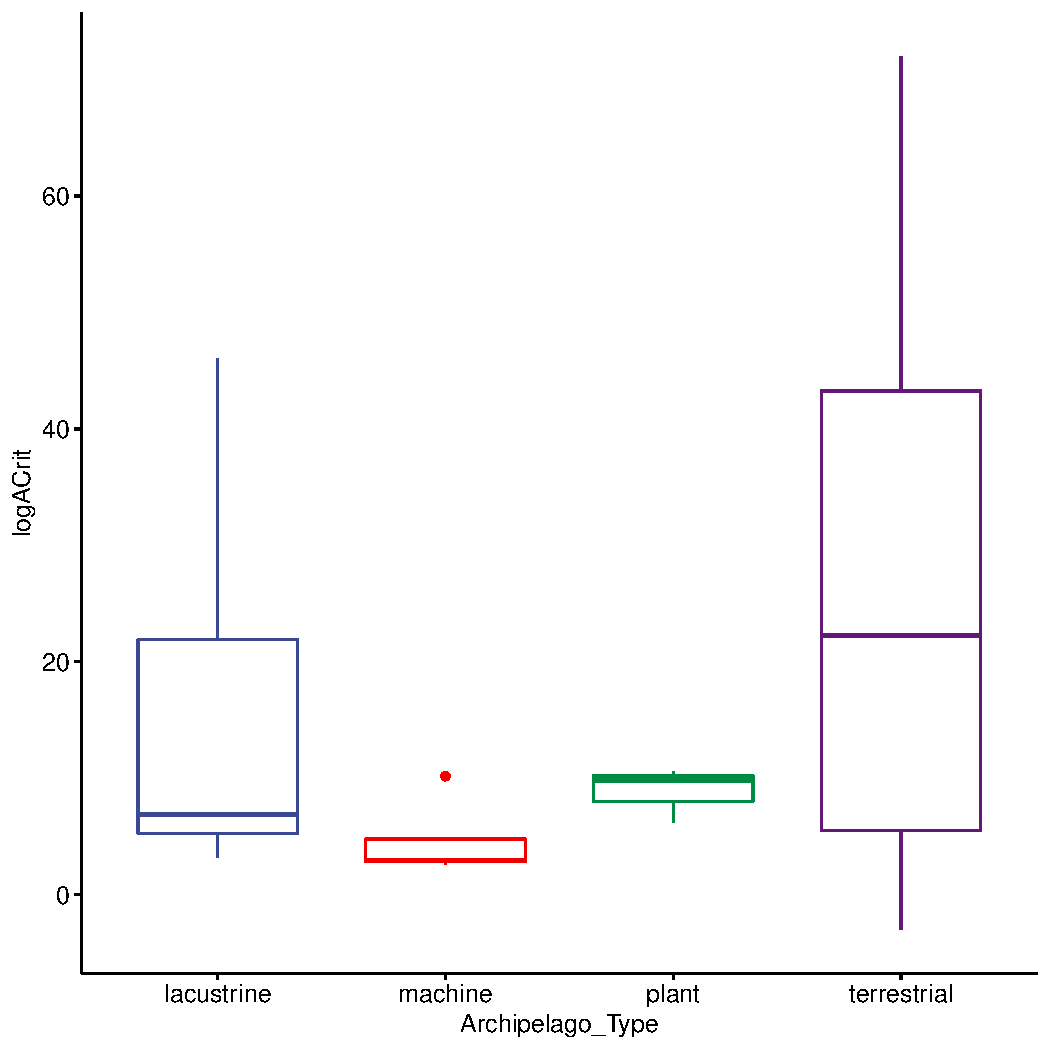
\includegraphics[width=.5\textwidth]{BoxplotTotalACritArch.pdf}\hfill
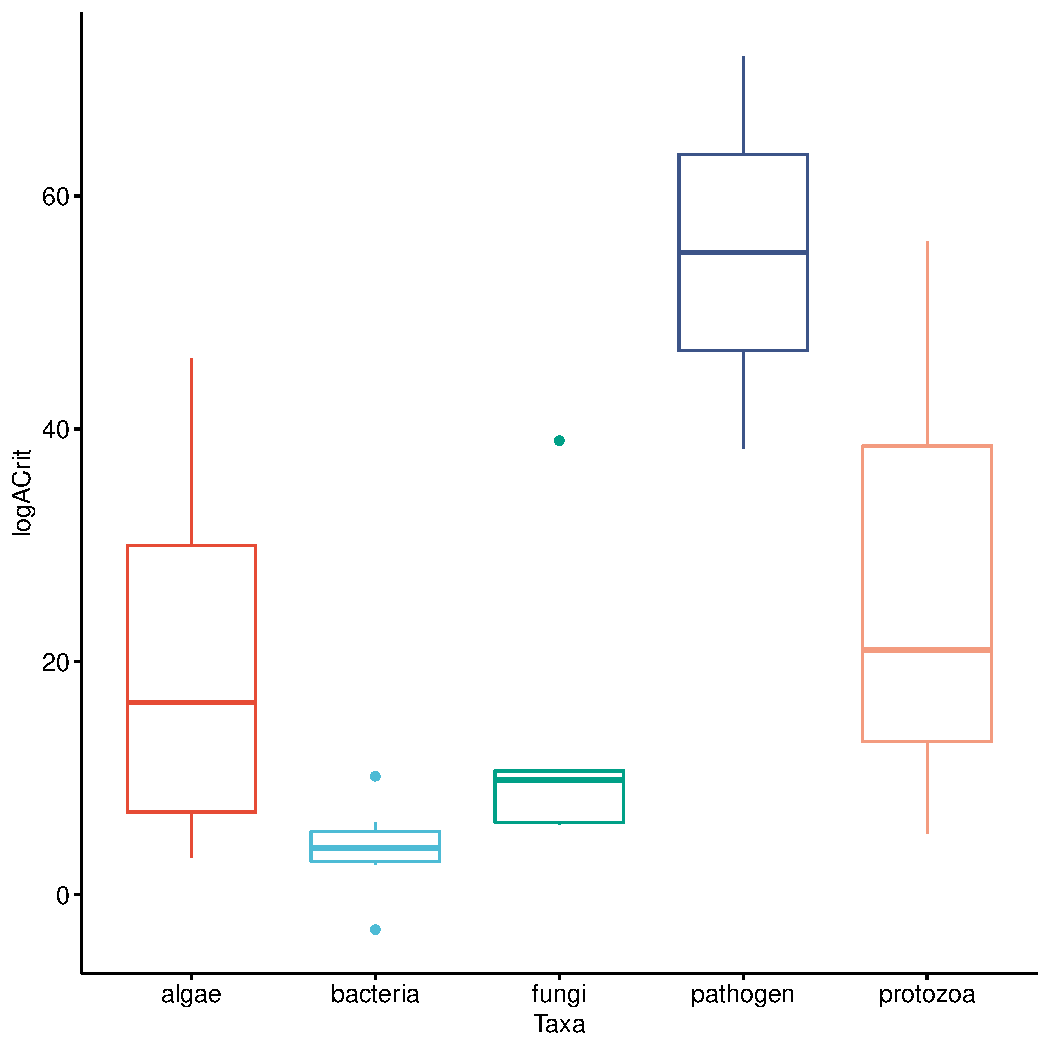
\includegraphics[width=.5\textwidth]{BoxplotTotalACritTaxa.pdf}\hfill

\hspace{10pt}\textbf{Habitat Type} \hspace{110pt} \textbf{Taxonomic Group}

\caption{log \textit{A\textsubscript{crit}} by habitat type and taxonomic group after removing anomalous result}
\label{fig:figure8}

\end{figure}


}

\begin{table}[h]
\begin{center}
    \caption{Table showing the results of multiple regression analysis of estimated effect of taxonomic group only on log \textit{A\textsubscript{crit}}}
    \label{crouch}
    \begin{tabular}{  l  p{1.5cm} p{3cm}  p{1.5cm}}
        \toprule
\textbf{Variable} 
&\textbf{Estimate}      
& \textbf{95\% CI}
& \textbf{p-value}   \\\midrule
intercept (algae)
&20.56
& [5.07, 36.07]
& 0.0121 \\\hline
taxonomic group
&
& 
&0.004 \\\hline
bacteria
&-16.500
& [-35.12, 2.12]
&0.0791 \\\hline
fungi
&-6.222 
& [-27.01, 14.56]
& 0.5373 \\\hline
pathogens
&34.587
& [7.75, 61.42]
& 0.0144 \\\hline
protozoa
&6.879 
& [-16.79, 30.55]
& 0.5491  \\
        \bottomrule
    \end{tabular}
    \end{center}
\end{table}









\chapter{Discussion}

%Discussion. This should attempt to tie together the results, what they indicate in a broader context, the extent to which the original aims have been satisfied and what future work is suggested. Return to and address the ideas raised in the introduction. In particular, think about:
%What’s the main thing we know now that we didn’t know before?
%What’s the chain of logic and results that means we know it?
%How does this affect our -- and other scientists’ -- view of the world? What are the implications?
%What are the implications of the intermediate steps in the chain towards the main thing?

%Plan:
%What have I essentially demonstrated? 

%DONE
I have presented three variations of the Chisholm model \cite{chisholm2016maintenance} that take into account varying habitats and immigration routes and have successfully fit all three to microbial TAR data. The relatively equal success of the three model variations (Classic, Depth, Perimeter) suggests that immigration route is not a significant factor in defining microbial TARs (see Supplementary Materials, Table 7.5).  Microorgansims can cross oceanic barriers via airborne dust particles \cite{rosselli2015microbial}, enter glacial habitats via stream deposition \cite{darcy2018island} and reach pole-to-pole via airborne, animal vector and anthropogenic mediated dispersal \cite{kleinteich2017pole}. Microbial OTUs likely utilise a variety of immigration routes when entering a new environment. No significant accuracy was lost in assessing three-dimensional habitats using the two-dimensional models (Classic, Perimeter), suggesting habitat depth did not affect OTU richness as strongly as area, where area acts as immigration portal into the three-dimensional habitat. Algae and bacteria have shown negative correlations between OTU richness and depth \cite{battes2019species} \cite{turner2017microbial}. These patterns emerge as increasing habitat depth often accompanies nutrient-poor, low-energy environments. The immigration portal may be characterised by a nutrient-rich, high-energy stratification that is a more potent predictor of OTU richness than depth. \\

%%%%talk about the power law model
%DONE
\noindent The phenomenological power-law model did not perform significantly better than the mechanistic Classic, Depth and Perimeter models, according to the AIC measure of parsimony, relative to model fit (see Supplementary Materials, Table 7.4). This indicates that the model parameters ($\theta$, \textit{m\textsubscript{0}}, \textit{K}, $\rho$) were useful in fully describing the shape of the observed TARs, thus supporting the hypothesis that OTU richness is influenced by the parameters, rather than being simply a constant power of the area. The mean slope of positive TARs across these datasets was comparable to macroorganisms (\textit{z}=0.16) and higher than those previously reported for microbial taxa \cite{rosenzweig1995species} \cite{green2004spatial} (see Supplementary Materials, Table 7.3). These observations show habitat area has a relatively strong influence on OTU richness. Isolated habitats may provide the stability needed for microbial taxa to reach equilibrium and for stronger TARs to arise, in contrast to turbulent continuous habitats \cite{bell2005larger}.    \\

%DONE
\noindent The successfully fitted datasets exhibit both the classic MacArthur and Wilson \cite{MacArthurRobertH1967Ttoi} biogeographic pattern of increasing OTU richness with area and the small island effect of OTU richness varying independently of area. The results demonstrate that some microbial communities are constrained by niche-structured regimes at smaller areas where immigration is low, before transitioning to colonisation-extinction balance regimes at larger areas where immigration is high. This lends support to the theory that microbial species are not ubiquitous and unlimited in dispersal, that they can be limited by habitat heterogeneity, resource availability and dispersal barriers, but this is not a ubiquitous pattern with over 50\% of the datasets failing to be fit by the model. \\

%DONE
\noindent Many datasets with positive TARs (as indicated by Spearman's rank correlation coefficients) could not be successfully fit with the power-law, Classic, Depth or Perimeter models (see Supplementary Materials, Figure 7.2). Despite positive \textit{z} values for these datasets, confidence intervals included zero and therefore were not statistically significant. Stochastic variation between data points inhibited the models from discerning significant TARs (see Supplementary Materials, Figure 7.2 a \& b). The majority of failed fits were aquatic habitats and may be due to uncertainty in the spatial sample regime of a heterogenous habitat. In order to elucidate the the spatial patterns within these habitats, it might be useful to take a stratified approach. Some of the failed fits had too few data points in comparison to the parameters of the model, producing low adjusted R\textsuperscript{2} values (see Supplementary Materials, Figure 7.2 b). Microbial TARs may also be undetected due to the disparity between sample and community sizes meaning rare taxa are missed \cite{woodcock2006taxa}.\\ 

%\noindent The majority of failed fittings were for aquatic habitats. For my successful fittings, aquatic groups such as algae and protozoa show wide ranging \textit{A\textsubscript{crit}} results suggesting their is uncertainty caused by spatial sampling regime in a spatially heterogenous environment.  Due to the data available and for computational simplicity, OTUs were considered evenly distributed throughout the water column, however, OTUs are subject to spatial heterogenous distributions throughout a three-dimensional habitat \cite{barberan2011euxinic}. In order to clearly elucidate TARs in any three-dimensional environment it may be necessary to quantifying OTU richness in each stratification separately in addition to analysing the habitat as a whole.   

%DONE
\noindent This project is, to the best of my knowledge, the first attempt to apply a biphasic mechanistic TAR model to microbial data. The model demonstrates that when niche diversity increases slowly or remains constant and immigration increases quickly with area, a biphasic TAR is produced. At an \textit{A\textsubscript{crit}} specific to that habitat and taxonomic group, the TAR will transition from deterministic to a stochastic mechanisms. I hypothesised that \textit{A\textsubscript{crit}} would be lower where immigration is higher (i.e. for more motile OTUs and less isolated habitats). My analysis indicated that taxonomic group was significant in predicting \textit{A\textsubscript{crit}}, while habitat type was not. It is likely that taxonomic group is significant in predicting \textit{A\textsubscript{crit}} as taxa are constrained (or liberated) by their own range of life cycles (activity and dormancy) and dispersal methods (sporulation, meteorological, biotic, anthropogenic, passive). According to this data isolated habitats present no significant dispersal barriers to microorganisms as a whole, although their relative accessibility varies between taxonomic groups.\\

%DONE
\noindent My analysis indicated that pathogenic OTUs had overwhelmingly higher \textit{A\textsubscript{crit}} values (mean 9.43 x 10\textsuperscript{30} cm\textsuperscript{2}), thus they are more constrained by resource availability and dispersal barriers. I suggest this is due to their dependence on host species, although this will be directly related to the motility and sociability of their hosts. The two datasets used in this study quantify human pathogen richness on 'true' islands \cite{jean2016equilibrium}. Human pathogen OTU richness is negatively correlated with disease control efforts \cite{dunn2010global}. I suggest that global mitigation strategies such as behavioural change, medicine and vaccination \cite{nicolaides2020hand} mean pathogens face considerable dispersal barriers that limit immigration and constrain them to niche-structured spatial regimes over larger areas. \\

%DONE
\noindent Bacterial OTUs exhibited the lowest mean \textit{A\textsubscript{crit}} value (3.02 x 10\textsuperscript{3} cm\textsuperscript{2}). The small size of bacteria allows them to dispersal more freely than size-limited macroorganisms \cite{martiny2006microbial}. They may also overcome dispersal limitation through dormancy as a biogeographical response and as a consequence of enormous population sizes \cite{LoceyKennethJ2010Stbw} \cite{fenchel2004ubiquity}. Bacteria have a variety of ecological traits that allow them to move freely and access isolated habitats, thus they transition to stochastic TAR mechanisms at lower areas. \\
 
 %DONE
\noindent Fungi also showed low \textit{A\textsubscript{crit}} values (mean 1.72 x 10\textsuperscript{16} cm\textsuperscript{2}). Mycorrhizal fungi, where there are beneficial associations with plant roots, have large spores that immigration slowly through soil \cite{bueno2019arbuscular}, however, the close proximity of potential host plants might mitigate low fungal motility. For other fungal groups, long distance spore dispersal is facilitated by meteorological, biotic and anthropogenic vectors \cite{golan2017long}. Fungal sporulation allows taxa to overcome local and regional barriers, thus contributing to the low \textit{A\textsubscript{crit}} values seen in these datasets. \\

%DONE
\noindent Algae (mean 2.56 x 10\textsuperscript{19} cm\textsuperscript{2}) and protozoa (mean 7.43 x 10\textsuperscript{23} cm\textsuperscript{2}) exhibited similar midrange \textit{A\textsubscript{crit}} values. The broad range of \textit{A\textsubscript{crit}} values for these taxonomic groups may be due to the issue of spatial sampling regime in spatially heterogenous aquatic environments. Issues of taxonomic classification, particularly for protists may contribute to varying estimations of diversity \cite{foissner2006biogeography}. Whilst seems that algae and protists transition from deterministic to stochastic mechanisms of spatial scaling in the midrange of areas, further investigation is needed to discern a true pattern within the wide range of  \textit{A\textsubscript{crit}} values estimated. The multiple regression model coefficients (Table 3.7) broadly confirm the overall taxonomic results. \\

%DONE
\noindent As the multiple regression analysis showed that habitat type was non-significant in predicting \textit{A\textsubscript{crit}} I cannot assess the relative isolation of habitats or how they may affect \textit{A\textsubscript{crit}}. It is interesting however to look at the mean \textit{A\textsubscript{crit}} values for each habitat type, as a sign post towards what may be found with a more comprehensive dataset. Terrestrial habitats show the highest mean \textit{A\textsubscript{crit}} values (2.36 x 10\textsuperscript{30} cm\textsuperscript{2}). This may be due to immigration via an accidental vector being limited to aerial species that can reach the land island. Passive immigration by water or air to land islands relies on stochastic success which may limit dispersal, although fungal and bacteria OTU richness has been shown be unaffected by isolation \cite{li2020island}. \\

%DONE
\noindent Lacustrine habitats exhibited low mean \textit{A\textsubscript{crit}} values (1.28 x 10\textsuperscript{19} cm\textsuperscript{2}) suggesting immigration to these habitats is high. Aquatic taxa such as algae and protozoa utilise a variety of dispersal mechanisms between habitats, including dispersal via insects and waterfowl \cite{stewart1966dispersal}. It may be easier for microbial OTUs to colonise inland lacustrine environments where animal activity increases the probability of transport via an accidental vector. Passive transport to lacustrine environments may have a greater success rate than terrestrial islands due to the interconnectivity of rivers and streams that empty into watershed areas, filling lakes and ponds.  

%DONE
\noindent Plant habitats also have low mean \textit{A\textsubscript{crit}} values (2.01 x 10\textsuperscript{4} cm\textsuperscript{2}). For many symbiotic plant-microbe species relationships, plant seeds are already inoculated with associated microbial taxa on dispersal \cite{ho2017plant}. Thus dispersal barriers between plant and microbes are removed, contributing to low \textit{A\textsubscript{crit}} values. Many plant communities are comprised of the same species in close proximity, providing ready access to source populations and increasing immigration. 

%DONE
Four of the six best-fit datasets were for bacteria in machine habitats (membrane bioreactors and metal cutting machine sump tanks) \cite{van2006bacterial} \cite{van2005island}. It may be that the strong TAR found in these environments is a function of their isolation, relative to natural habitats. Despite the large numbers, rapid asexual reproduction and resilience to extinction of bacteria, when constrained by immigration, more prominent and easily quantifiable TAR patterns arise. The model fitting process supports this by estimating extremely low immigration rates for machine habitats. Despite this, machine habitats had the lowest mean \textit{A\textsubscript{crit}} (6.56 x 10\textsuperscript{3} cm\textsuperscript{2}). \textit{A\textsubscript{crit}} is not only affected by immigration as in my primary hypothesis, but can also be affected by number of niches (\textit{K}), density ($\rho$) and $\theta$. In the fitted model the low \textit{A\textsubscript{crit}} for machine habitats in spite of their isolation is caused by the low \textit{K} values of homogenous, man-made environments, a characteristic of these unusual habitats that warrants further investigation. \\
%DONE
\noindent The non-significance of habitat type, despite marked differences in the mean \textit{A\textsubscript{crit}} is due to the large, overlapping estimate ranges. Overall, after removing the outlying datapoint and removing habitat type as an explanatory variable, the model accounts for nearly half of the variation in log \textit{A\textsubscript{crit}} using the broad taxonomic groups.\\


%\noindent The results of this investigation support the theory that critical area will be larger for pathogens  and lower for bacteria (3.02 x 10\textsuperscript{3} cm\textsuperscript{2}), but protozoan critical area (7.43 x 10\textsuperscript{23} cm\textsuperscript{2}) was higher than algae (2.56 x 10\textsuperscript{19} cm\textsuperscript{2}) or fungi (1.72 x 10\textsuperscript{16} cm\textsuperscript{2}), in contrast to my prediction. 

%As habitat type was not significant in predicting log \textit{A[\textsubscript{crit}} I cannot address the hypothesis that more isolated habitats will have lower log \textit{A[\textsubscript{crit}}. Examination of the mean differences between habitats suggests that terrestrial habitats showed higher critical area (2.36 x 10\textsuperscript{30} cm\textsuperscript{2}) than lacustrine (1.28 x 10\textsuperscript{19} cm\textsuperscript{2}) and plant habitats (2.01 x 10\textsuperscript{4} cm\textsuperscript{2}) as predicted, but machine habitats had a lower critical area than expected (6.56 x 10\textsuperscript{3} cm\textsuperscript{2}). 

%Which datasets were successfully fit to the model and why? What do they have in common? Where do they differ in terms of habitat, taxonomic group and study design. 

%Which datasets weren't successfully fit to the model and why?


%Why did the riverine habitat and archaea taxa not have any successful fittings?
%DONE
\noindent The reason for the lack of successful fittings for riverine habitats is due to the low number of data points in each of these studies (see Table 7.1, Supplementary Material). Whilst the majority of these datasets had high R\textsuperscript{2} values, once adjusted R\textsuperscript{2} values were calculated the fittings were unsuccessful. Only one dataset included archaeal TARs and no significant relationship between area and OTU richness was found. This is likely due to the importance of environmental filtering for extremophile OTUs in soda lakes \cite{LanzenAnders2013SPaE}. It is interesting to note other datasets removed from the fitting process due to a lack of positive TARs. These included, fungi in the Antarctic cryoconite holes of two glaciers where extreme biomass influx negated observable TARs (datasets 10 \& 11) \cite{darcy2018island}. Inappropriate diversity metrics and spatial scaling may have led to undetectable toot-symbiotic fungi TARs (dataset 18) \cite{davison2018microbial}. Fungi OTU richness did not increase with area on submerged leaves due to a lack of energy increase with corresponding area as expressed by the species-energy theory (dataset 39) \cite{FeinsteinLarryM2012Tran}  \cite{wright1983species}. TARs may not have arisen in protozoan communities in submerged substrate due to a failure to reach equilibrium (dataset 55) \cite{henebry1980effect}. It is clear that the factors affecting microbial TARs are diverse and each habitat/taxa pairing may require unique assessment. \\ 

%DONE
%What was the anomalous result? Why was it anomalous?
\noindent The anomalous result removed from analysis concerned pathogenic bacterial OTU richness on 'true' geographic islands \cite{jean2016equilibrium}. The model was a poor fit to the data (R\textsuperscript{2}=0.23, adjusted R\textsuperscript{2}=0.18) and it's likely the error associated with estimating density for pathogenic bacteria over such large geographic scales lead to poor estimations of the remaining parameters and an excessive critical area estimate.   \\

%DONE
%What are the caveats that apply to this study? (Leave out caveats that apply to all studies.)
\noindent Whilst the data here indicate that habitat type is non-significant in predicting log \textit{A\textsubscript{crit}}, the large variation in mean log \textit{A\textsubscript{crit}} suggests there many be too few data points to discern a significant pattern. I also encountered challenges when trying to compare studies that used a variety of methods and quantification techniques. Microbial OTUs inhabit three-dimensional habitats and whilst steps have been taken here to account for this there is more work to be done to incorporating this fully. In a future extension of this mode I would consider each stratification of a habitat separately, to account for spatial heterogeneity. Volume has been shown to be more accurate in quantifying microbial TARs \cite{van2006bacterial}. It would be useful to further modify the model to explicitly incorporate volume and \textit{V\textsubscript{crit}} across datasets, as nearly all of them concern habitats within a volume even though often only surface area data is provided. Here I have used area with a depth metric (Depth Model) which suggests the habitat maintains the same area for the full depth, whereas natural habitats rarely take this shape and this reduces the accuracy of my results. \\

%DONE
\noindent Another issue I encountered was density estimations. The model required an estimation of individual density per unit area, however, direct counts are rarely given for microbial OTUs. Estimations were made in various ways, using gene sequence numbers or proxy papers, although these methods introduce error into the model fitting process. It would be beneficial to this project to develop more robust methods for estimating density as data taken from proxy papers introduces error into the fitting process. A broad scale experiment to quantify microbial TARs in a laboratory, where data specific to the needs of these model could be collected (i.e. density), could provide a more vigorous assessment of the models applicability to microbial TARs. \\

%DONE
\noindent When validating my model fitting procedures, error between true and estimated results increased with increasing parameter values. As I increased simulation parameters in parallel with each other (e.g. an increase in $\theta$,  was coupled by an increase in \textit{m\textsubscript{0}} and \textit{K}), the source of the increasing error is difficult to discern. Parameter ranges of speciation rate, \textit{m\textsubscript{0}} and \textit{k} given to the simulations were not inferred from microbial ecological theory, but were selected for ease of computation. A more thorough exploration of the parameter space, with ecologically relevant parameter ranges, to further validate the model fitting procedure and the areas of parameter space where there may be errors in fitting would be desirable in further work. \\

%What might be done about them? (Very important in a project write-up -- What would you do differently if you were doing the project again or had more time?)

%What future work could build more broadly on what we’ve found?
%DONE
\noindent There remains to be a thorough synthesis between biogeography and microbial ecology. Here I have gone some way to evaluate the influence of immigration on microbial TARs, however more work is needed to examine dispersal barriers. Dormancy is a widespread microbial response that may allow OTUs to overcome dispersal barriers and increase immigration to new habitats. However, it is a slow, passive process that will not necessarily lead the individual to a viable habitat \cite{LoceyKennethJ2010Stbw}. To fully elucidate the interplay of microbial ecology and biogeographic patterns, work is needed to incorporate dormancy as a biogeographic response.  \\         

%What are the implications of this work?
%DONE
\noindent An implication of this work is that if we can identify the niches within a habitat and the taxonomic groups that tend to occupy those niches, we may be able to better predict OTU richness at a range of spatial scales. This presents a complex challenge that requires the integration of environmental variables and habitat stratification. If these challenges could be overcome, it would be a particularly useful tool in predicting colonisation of new habitats such as soil exposed by glacier retreat, thus helping us model the biogeochemical processes this colonisation will produce. \\      

%A nice wrap-up, emphasising how this study in this system is of interest to people who work on other things, or other systems.
\noindent This study has demonstrated that microbial communities in isolated 'island' habitats can be subject to deterministic biogeographic mechanisms such as niche-structuring, before a critical area of transition (\textit{A\textsubscript{crit}}), to stochastic mechanisms of colonisation and extinction. I have also shown that taxonomic group is significant in predicting \textit{A\textsubscript{crit}}, but habitat type is not. The overwhelming number and complexity of microbial life, as well as the vital role these organisms play in ecosystem functioning, illustrates the importance of elucidating their biogeographic patterns. I hope that my study will lead to further research into the presence of deterministic and stochastic mechanisms in microbial biogeography, as well as the importance of taxonomic group on the relative influence of these processes. The synthesis of microbial ecology and biogeography will be of increasing interest as climate change alters habitats, creating and removing barriers, extending the range of pathogenic OTUs and leading to climate feedback loops of mineral and nutrient cycling. Microbial biogeography is an essential area of study in our global challenge to predict and mitigate the impacts of climate change. Everything is \textit{not} everywhere, and everything is changing.             
\chapter{Data and Code Availability}

Name a data (e.g., Dropbox, FigShare, Zenodo, etc) and a code (e.g., Dropbox, GitHub, etc.) archive from where the data and code can be obtained that will allow replication of your results. The code may be in the form of a single script file. You will be taught the principles of reproducible analyses in the R week of your coursework. If the data cannot be made available publicly (e.g., because it is yet to be formally published), or if there are some other confidentiality issues with submitting the data, speak with your course director and supervisor, and include a clear statement about why the data cannot be made available under the same Code and Data Availability header. Note that most data repositories allow timed embargos on data (e.g., Zenodo; see http://about.zenodo.org/policies/).
\chapter{Acknowledgements}
Thank you to my supervisors, Ryan, James and Tom. Thank you to all of the people that took the time to share their data with me.

\bibliographystyle{apalike}
\bibliography{bibliography}
\addcontentsline{toc}{chapter}{Bibliography}


\chapter{Supplementary Material}

%\begin{figure}
%\includegraphics[width=1\textwidth]{RhoShortPic.png}
%\end{figure}

 \begin{figure}[h!]
\centering
  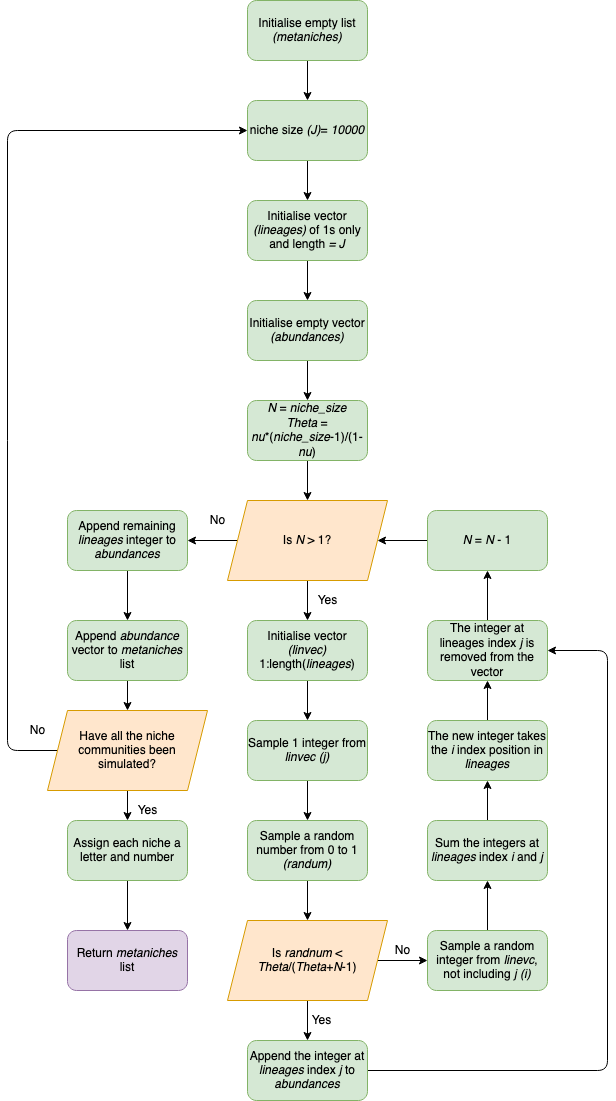
\includegraphics[scale=0.4]{metacommunity.png}
  \caption{Flowchart of metacommunity function}
  \label{fig:Flowchart}
\end{figure}

\begin{table}[h]
    \caption{Summary of Datasets}
    \label{crouch}
    \begin{tabular}{  l  p{5cm} p{1.5cm}  p{3cm} p{3cm}}
        \toprule
\textbf{Study and Dataset ID} 
&\textbf{Author and Year}      
& \textbf{Habitat}
& \textbf{Taxa}   \\\midrule
Study 1, Datasets 1 \& 2
&\cite{li2020island}
& Terrestrial
& Bacteria \& Fungi \\\hline
Study 2, Dataset 3
&\cite{battes2019species} 
& Lacustrine
&Algae \\\hline
Study 3, Datasets 4-15
&\cite{darcy2018island} 
& Lacustrine
&Bac, Alg, Fungi \& Proto \\\hline
Study 4, Datasets 16 \& 17
&\cite{delgado2018experimentally} 
& Terrestrial
& Bacteria \\\hline
Study 5, Dataset 18
&\cite{davison2018microbial} 
& Terrestrial
& Fungi \\\hline
Study 6, Datasets 19 \& 20
&\cite{glassman2017theory} 
& Plant
& Fungi \\\hline
Study 7, Dataset 21
&\cite{varbiro2017functional} 
& Lacustrine
& Algae \\\hline
Study 8, Datasets 22 \& 23
&\cite{kavazos2016small} 
& Lacustrine
& Bac \& Proto \\\hline
Study 9, Dataset 24
&\cite{bolgovics2016species} 
& Lacustrine
& Algae \\\hline
Study 10, Datasets 25-27
&\cite{article} 
& Lacustrine
& Alg, Proto \& Fun \\\hline
Study 11, Datasets 28-32
&\cite{jean2016equilibrium} 
& Terrestrial
& Bac, Path, Fun \& Proto \\\hline
Study 12, Dataset 33
&\cite{cashdan2014biogeography} 
& Terrestrial
& Pathogens \\\hline
Study 13, Dataset 34
& \cite{LepereCecile2013Gdae}
& Lacustrine
&Protozoa \\\hline
Study 14, Datasets 35 \& 36
& \cite{LanzenAnders2013SPaE}
& Lacustrine
& Bacteria \& Archaea \\\hline
Study 15, Dataset 37
&\cite{RENGEFORSK2012Plma} 
& Lacustrine
& Algae \\\hline
Study 16, Datasets 38-39
&\cite{FeinsteinLarryM2012Tran} 
& Plant
& Fungi \\\hline
Study 17, Dataset 40
&\cite{StompMaayke2011Lbpi} 
& Lacustrine
& Algae \\\hline
Study 18, Dataset 41
&\cite{JohnL.Orrock2011BaER} 
& Terrestrial
& Pathogens \\\hline
Study 19, Datasets 42 \& 43
&\cite{barberan2011euxinic} 
& Lacustrine
& Bacteria \\\hline
Study 20, Dataset 44
&\cite{peay2007strong} 
& Plant
& Fungi \\\hline
Study 21, Dataset 45
&\cite{van2006bacterial} 
& Machine
& Bacteria \\\hline
Study 22, Dataset 46
&\cite{bell2005larger} 
& Lacustrine
& Bacteria \\\hline
Study 23, Dataset 47
&\cite{reche2005does} 
& Lacustrine
& Bacteria \\\hline
Study 24, Datasets 48-50
&\cite{van2005island} 
& Machine
& Bacteria \\\hline
Study 25, Dataset 51
&\cite{karatayev2005community} 
& Lacustrine
& Algae \\\hline
Study 26, Datasets 52 \& 53
&\cite{mccormick1988comparison} 
& Riverine
& Protozoa and Algae \\\hline
Study 27, Dataset 54
&\cite{wildman1987fungal} 
& Terrestrial
& Fungi \\\hline
Study 28, Dataset 55
&\cite{henebry1980effect} 
& Lacustrine
& Protozoa \\\hline
Study 29, Datasets 56 \& 57
&\cite{patrick1967effect} 
& Riverine
& Algae \\
        \bottomrule
    \end{tabular}
\end{table}

\begin{table}[h]
    \caption{Rho Estimation Methods (S \& D ID = Study \& Dataset ID)}
    \label{crouch}
    \begin{tabular}{  l  p{2cm} p{2cm}  p{1.5cm} p{5cm} p{5cm}}
        \toprule
\textbf{Study/Data}   
&\textbf{Taxa}
&\textbf{Habitat}   
& \textbf{$\rho$ (cm\textsuperscript{3})}   
& \textbf{Method} \\\midrule
S1, D1 
& Bacteria
& Soil
& 1.48x10\textsuperscript{12}   
& Gene seq num from paper \\\hline
S1, D2   
& Fungi
& Soil
& 7.41x10\textsuperscript{3}              
& Gene seq num from paper \\\hline
S2, D3  
&Algae
&Freshwater
& 3.56x10\textsuperscript{3}   
& Proxy \cite{pasztaleniec2010phytoplankton} \\\hline
S3, D4-6  
&Bacteria
&Cryo Holes
& 4.50x10\textsuperscript{4}   
& Proxy \cite{cameron2012structure} \\\hline
S3, D7-9  
&Algae
&Cryo Holes
& 1 
& Gene seq num from paper \\\hline
S3, D10-12  
&Fungi
&Cryo Holes
& 1  
& Gene seq num from paper \\\hline
S3, D13-15  
&Protozoa
&Cryo Holes
& 1   
& Gene seq num from paper \\\hline
S4, D16 
&Bacteria
&Soil
& 3.50x10\textsuperscript{12} 
& Gene seq num from paper \\\hline
S4, D17 
&Bacteria
&Soil
& 1.48x10\textsuperscript{13}  
& Gene seq num from paper \\\hline
S5, D18 
&Fungi
&Soil
& 1     
& 1 as area includes entire island \\\hline
S6, D19 \& 20 
&Fungi
&Soil
& 2.98x10\textsuperscript{3}   
& Gene seq num from paper \\\hline
S7, D21 
&Algae
&Freshwater 
& 3.56x10\textsuperscript{3}   
& Same proxy as D3 \\\hline
S8, D22
&Bacteria
&Sal Water
& 3.00x10\textsuperscript{6}    
& Proxy \cite{anton2000extremely} \\\hline
S8, D23 
&Protozoa
&Sal Water
& 1.84x10\textsuperscript{2}          
& Proxy \cite{elloumi2006composition} \\\hline
S9, D24 
&Algae
&Freshwater 
& 3.56x10\textsuperscript{3}               
& Same proxy as D3 \\\hline
S10, D25 
&Algae 
&Freshwater
& 3.56x10\textsuperscript{3}             
& Same proxy as D3 \\\hline
S10, D26 
&Protozoa
&Freshwater 
& 1.92x10\textsuperscript{3}      
& Proxy \cite{olive2020control} \\\hline
S10, D27
&Fungi
&Freshwater
& 1         
& Proxy \cite{wurzbacher2010fungi} \\\hline
S11, D28-32
&Bac, Pat, Fun, Pro
&Hosts
& 1            
& 1 as area includes entire island \\\hline
S12, D33
&Pathogens
&Hosts
& 1        
& 1 as area includes entire island \\\hline
S13, D34
&Protozoa
&Freshwater 
& 5.72x10\textsuperscript{3} 
& Nanoflag count taken from paper \\\hline
S14, D35
&Archaea
&Sal Water
& 1.00x10\textsuperscript{7} 
& Book \cite{kulkarni2019alkaliphiles} \\\hline
S14, D36
&Bacteria
&Sal Water 
& 6.00x10\textsuperscript{6} 
& Proxy \cite{humayoun2003depth} \\\hline
S15, D37
&Algae
&Sal Water
& 4.85x10\textsuperscript{3} 
& Proxy \cite{rengefors2008marine} \\\hline
S16, D38-39
&Fungi
&Plant
& 10       
& No proxy found so 10 est \\\hline
S17, D40
&Algae
&Freshwater
& 3.56x10\textsuperscript{3}   
& Same proxy as D3 \\\hline
S18, D41
&Pathogens
&Hosts
& 1     
& 1 as area includes entire island \\\hline
S19, D42 \& 43
&Bacteria
&Freshwater
& 1.16x10\textsuperscript{7} 
& Proxy \cite{cole1993bacterial} \\\hline
S20, D44
&Fungi
&Soil
& 6.90x10\textsuperscript{6} 
& Proxy \cite{prevost2011validation} \\\hline
S21, D45
&Bacteria
&Machine
& 2.29x10\textsuperscript{10} 
& Cell abund taken from paper \\\hline
S22, D46
&Bacteria
&Tree Holes
& 4.90x10\textsuperscript{5} 
& Proxy \cite{rivett2018abundance} \\\hline
S23, D47
&Bacteria
&Freshwater
& 1.16x10\textsuperscript{7} 
& Same proxy as D43 \\\hline
S24, D48-50
&Bacteria
&Machine
& 2.29x10\textsuperscript{10}  
& Same proxy as D46 \\\hline
S25, D51
&Algae
&Freshwater
& 3.56x10\textsuperscript{3}    
& Same proxy as D3 \\\hline
S26, D52
&Protozoa
&River
& 5.72x10\textsuperscript{3} 
& Same proxy as D34 \\\hline
S26, D53
&Algae
&River
& 3.56x10\textsuperscript{3}    
& Same proxy as D3 \\\hline
S27, D54
&Fungi
&Soil
& 1.00x10\textsuperscript{5} 
& Book \cite{pepper2019biotic} \\\hline
S28, D55
&Protozoa
&Freshwater
& 5.72x10\textsuperscript{3} 
& Same proxy as D34 \\\hline
S29, D56 \& 57
&Algae
&River 
& 3.56x10\textsuperscript{3}   
& Same proxy as D3 \\
        \bottomrule
    \end{tabular}
\end{table}

\begin{figure}[htbp]
\centering
\subfloat[Dataset 4, bacteria in Antarctic Croconite Holes]{\label{fig:a}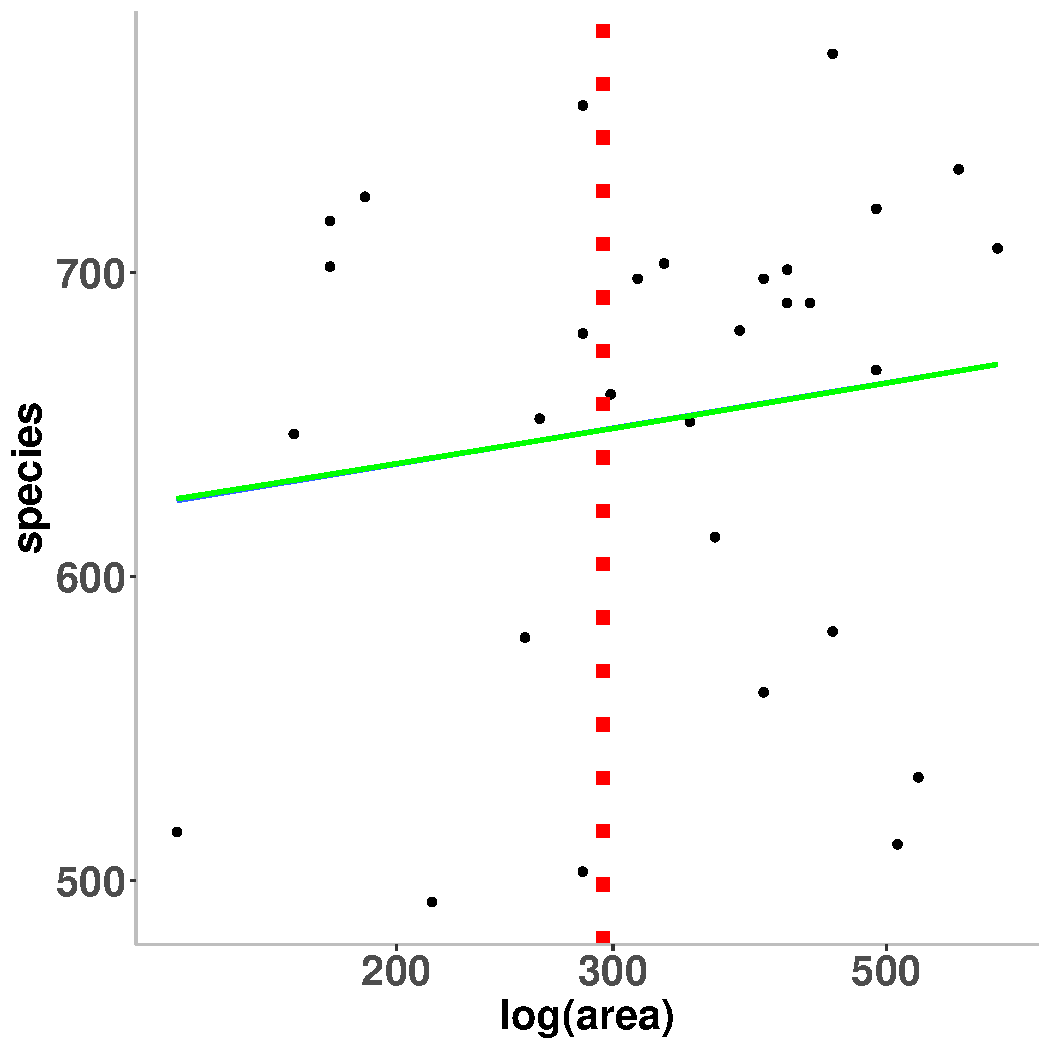
\includegraphics[width=0.45\linewidth]{../Results/ClassicNLLSPlot4.pdf}}\qquad
\subfloat[Dataset 54, fungi in a soil based laboratory experiment]{\label{fig:b}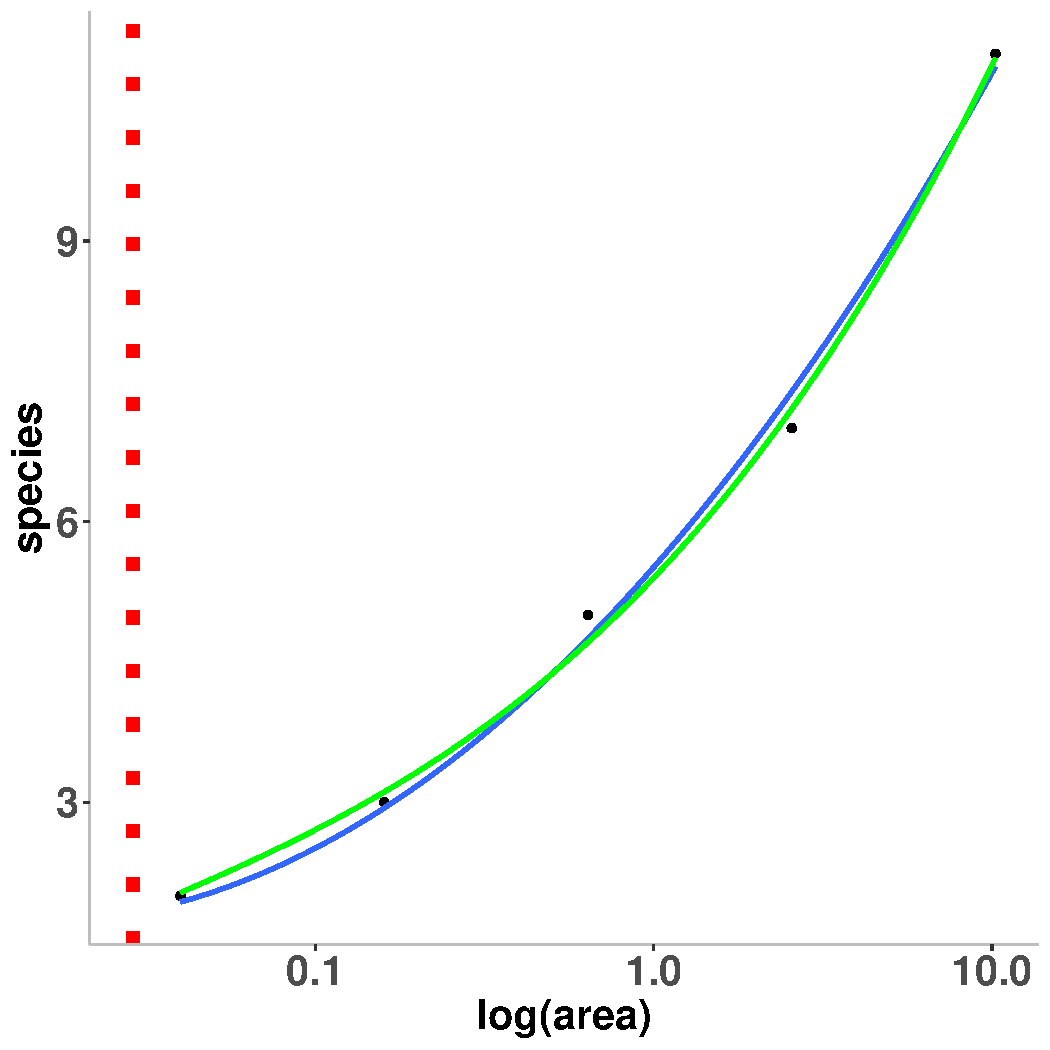
\includegraphics[width=0.45\linewidth]{../Results/PeriNLLSPlot48.pdf}}\\
\subfloat[Dataset 22, benthic bacteria in saline lakes (log area plotted with depth)]{\label{fig:c}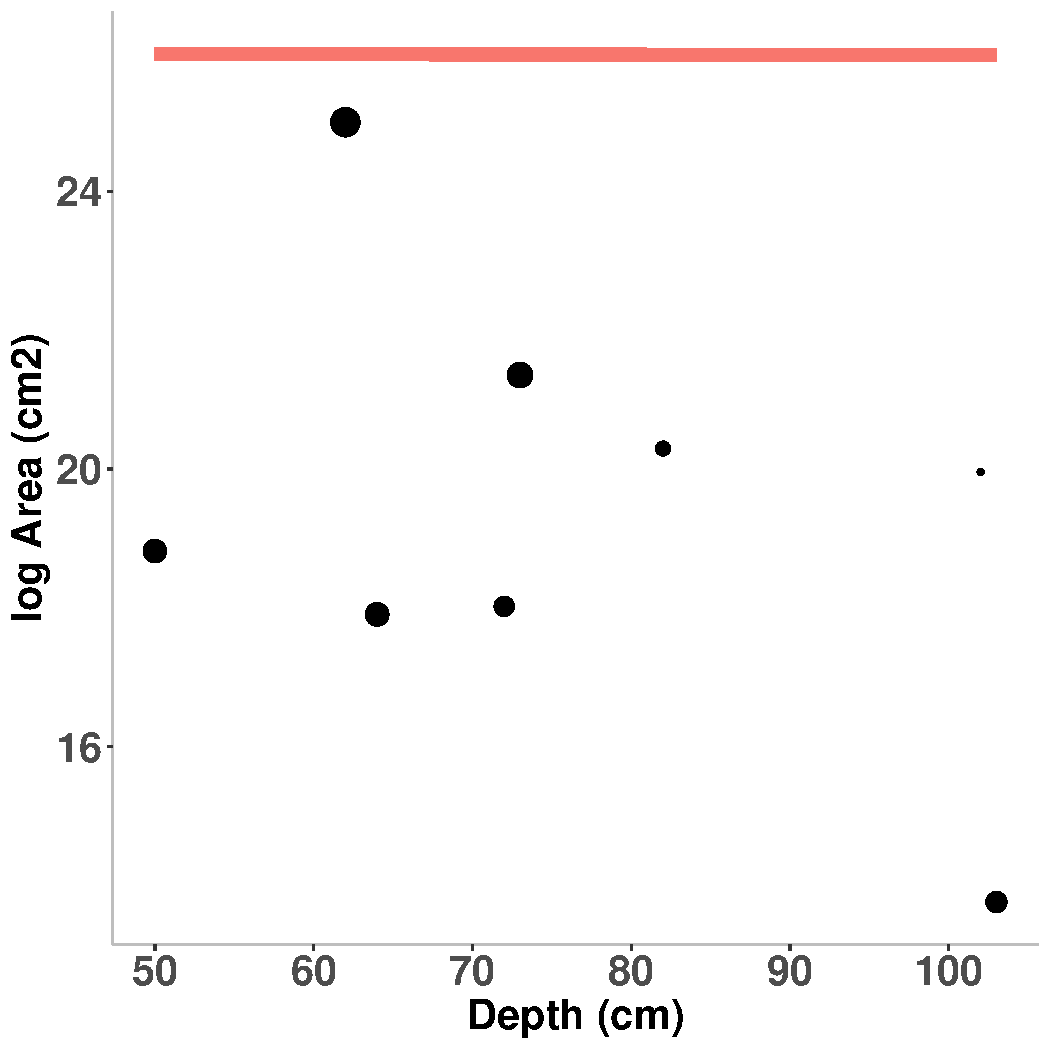
\includegraphics[width=0.45\textwidth]{../Results/DepthNLLSPlot19.pdf}}\qquad%
\subfloat[Dataset 22, benthic bacteria in saline lakes (log volume plotted with OTU richness)]{\label{fig:d}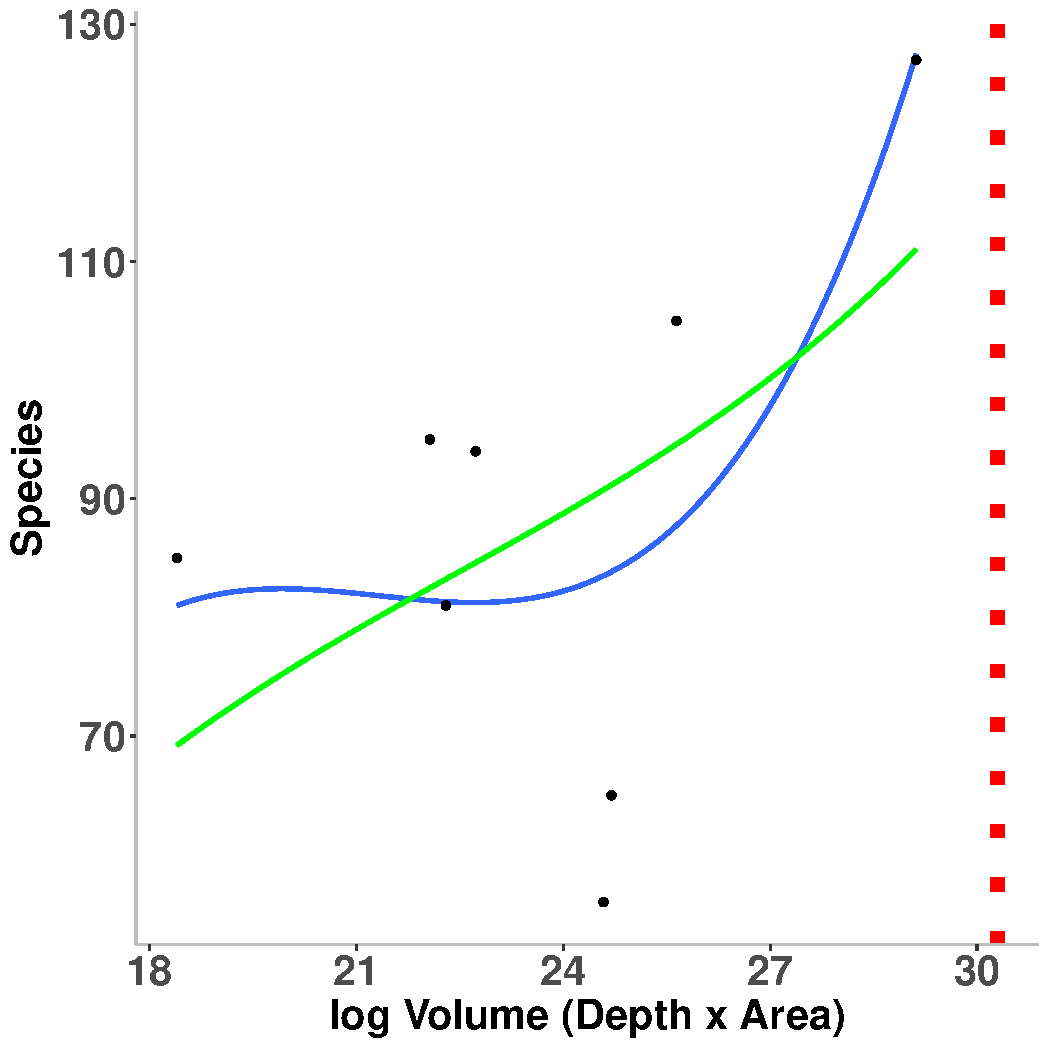
\includegraphics[width=0.45\textwidth]{../Results/DepthNLLSPlot2_19.pdf}}%
\caption{Selection of plots of datasets that failed to be fit using either of the three model variants (Classic, Depth, Perimeter) or the power-law model, where the blue line is the model fit, the green line is the power-law model fit and the red dotted line is the \textit{A\textsubscript{crit}} estimation. A) Dataset 4, bacteria in cryoconite holes with the Classic Model (R\textsubscript{2}=0.02, adjusted R\textsubscript{2}=-0.13, $\theta$=29, \textit{m\textsubscript{0}}=0.208, \textit{K}=354, \textit{A\textsubscript{crit}}=294 cm\textsuperscript{2}). B) Fungi in soil based laboratory experiment plotted with the Perimeter Model (R\textsubscript{2}=0.099, adjusted R\textsubscript{2}=Inf, $\theta$=6, \textit{m\textsubscript{0}}=6.24 x 10\textsuperscript{-6}, \textit{K}=1, \textit{A\textsubscript{crit}}=2.89 x 10\textsuperscript{-2} cm\textsuperscript{2}). C) Benthic bacteria in saline lakes plotted with the Depth Model (R\textsubscript{2}=0.51, adjusted R\textsubscript{2}=-0.15, $\theta$=14, \textit{m\textsubscript{0}}=1.98 x 10\textsuperscript{-16}, \textit{K}=81, \textit{A\textsubscript{crit}}=1.89 x 10\textsuperscript{11} cm\textsuperscript{2})}
\label{fig:myfig}
\end{figure}


\begin{table}[h]
    \caption{Results of successful Power-Law Model fitting to the 24 positive TAR datasets with R\textsuperscript{2}, adjusted R\textsuperscript{2}, \textit{z} values (model exponent), \textit{c} values (model constant) (S \& D ID = Study \& Dataset ID)}
    \label{crouch}
    \begin{tabular}{  l  p{6cm} p{1cm}  p{1cm} p{1cm} p{1cm}}
        \toprule
\textbf{S \& D ID} 
&\textbf{Author \& Year}
&\textbf{R\textsuperscript{2}}      
& \textbf{Adj R\textsuperscript{2}}
& \textit{z}  
& \textit{c}\\\midrule
S1, D1
&\cite{li2020island}
& 0.56
& 0.49
& 0.09
& 1294.63 \\\hline
S1, D2
&\cite{li2020island}
& 0.60
& 0.53
& 0.10
& 332.03 \\\hline
S3, D6
&\cite{darcy2018island} 
& 0.23
& 0.10
& 0.32
& 70.02 \\\hline
S3, D11
&\cite{darcy2018island} 
& 0.27
& 0.15
& 0.42
& 4.68\\\hline
S4, D16
&\cite{delgado2018experimentally} 
& 0.82
& 0.75
& 0.11
& 340.96 \\\hline
S4, D17
&\cite{delgado2018experimentally} 
& 0.70
& 0.54
& 0.08
& 451.61 \\\hline
S6, D19
&\cite{glassman2017theory} 
& 0.23
& 0.02
& 0.27
& 0.48 \\\hline
S6, D20
&\cite{glassman2017theory} 
& 0.32
& 0.13
& 0.16
& 1.93 \\\hline
S7, D21
&\cite{varbiro2017functional} 
& 0.02
& 0.0001
& 0.01
& 23.10 \\\hline
S9, D24
&\cite{bolgovics2016species} 
& 0.62
& 0.48
& 0.05
& 32.25 \\\hline
S10, D25
&\cite{article} 
& 0.38
& 0.28
& 0.06
& 48.28 \\\hline
S10, D26 
&\cite{article} 
& 0.29
& 0.17
& 0.14
& 0.29 \\\hline
S11, D28
&\cite{jean2016equilibrium} 
& 0.23
& 0.18
& 0.01
& 39.29 \\\hline
S11, D29
&\cite{jean2016equilibrium} 
& 0.34
& 0.30
& 0.02
& 19.31 \\\hline
S11, D30
&\cite{jean2016equilibrium} 
& 0.24
& 0.19
& 0.02
& 4.27 \\\hline
S11, D31 
&\cite{jean2016equilibrium} 
& 0.35
& 0.31
& 0.03
& 4.60 \\\hline
S11, D32
&\cite{jean2016equilibrium} 
& 0.33
& 0.29
& 0.05
& 4.26 \\\hline
S20, D44
&\cite{peay2007strong} 
& 0.87
& 0.78
& 0.18
& 0.64 \\\hline
S21, D45
&\cite{van2006bacterial} 
& 0.94
& 0.82
& 0.27
& 0.88 \\\hline
S22, D46
&\cite{bell2005larger} 
& 0.46
& 0.38
& 0.33
& 1.74 \\\hline
S24, D48
&\cite{van2005island} 
& 0.73
& 0.63
& 0.36
& 1.25 \\\hline
S24, D49
&\cite{van2005island} 
& 0.84
& 0.76
& 0.32
& 1.80 \\\hline
S24, D50
&\cite{van2005island} 
& 0.80
& 0.73
& 0.36
& 1.34 \\\hline
S25, D51
&\cite{karatayev2005community} 
& 0.10
& 0.09
& 0.11
& 19.00  \\
        \bottomrule
    \end{tabular}
\end{table}

\begin{table}[h]
    \caption{Results of Power-Law Model AIC score - Classic, Depth and Perimeter AIC scores. There must be a difference of at least 2 to be statistically significant (positive results favour the Classic, Depth and Perimeter Models, negative results favour the Power-Law Model) (S \& D ID = Study \& Dataset ID)}
    \label{crouch}
    \begin{tabular}{  l  p{6cm} p{1cm}  p{1cm} p{1cm} p{1cm}}
        \toprule
\textbf{S \& D ID} 
&\textbf{Author \& Year}
&\textbf{Classic}      
& \textbf{Depth}
& \textbf{Perimeter} \\\midrule
S1, D1
&\cite{li2020island}
& 7.25
& 7.25
& 6.91 \\\hline
S1, D2
&\cite{li2020island}
& 10.37
& 10.18
& 9.49 \\\hline
S3, D6
&\cite{darcy2018island} 
& 0.23
& 0.23
& 0.08 \\\hline
S3, D11
&\cite{darcy2018island} 
& 0.005
& 0.02
& 0.02\\\hline
S4, D16
&\cite{delgado2018experimentally} 
& 0.005
& 0.005
& 0.005 \\\hline
S4, D17
&\cite{delgado2018experimentally} 
& 0.002
& 0.002
& 0.002 \\\hline
S6, D19
&\cite{glassman2017theory} 
& 0.03
& 0.03
& 0.01 \\\hline
S6, D20
&\cite{glassman2017theory} 
& 0.72
& 0.72
& 0.52 \\\hline
S7, D21
&\cite{varbiro2017functional} 
& 1.20
& 1.22
& 1.03 \\\hline
S9, D24
&\cite{bolgovics2016species} 
& 2.64
& 2.62
& 3.33 \\\hline
S10, D25
&\cite{article} 
& 0.91
& 1.03
& 0.92 \\\hline
S10, D26 
&\cite{article} 
& 0.05
& 0.11
& 0.04 \\\hline
S11, D28
&\cite{jean2016equilibrium} 
& 0.49
& 0.49
& -0.61 \\\hline
S11, D29
&\cite{jean2016equilibrium} 
& 0.33
& 0.34
& 0.11 \\\hline
S11, D30
&\cite{jean2016equilibrium} 
& 2.77
& 2.78
& 3.16 \\\hline
S11, D31 
&\cite{jean2016equilibrium} 
& 0.76
& 0.75
& -0.05 \\\hline
S11, D32
&\cite{jean2016equilibrium} 
& 2.22
& 2.21
& 0.75 \\\hline
S20, D44
&\cite{peay2007strong} 
& -0.05
& -0.05
& -0.27 \\\hline
S21, D45
&\cite{van2006bacterial} 
& 2.67
& 2.67
& 2.25 \\\hline
S22, D46
&\cite{bell2005larger} 
& 0.45
& 1.34
& 0.17 \\\hline
S24, D48
&\cite{van2005island} 
& 2.84
& 2.87
& 0.47 \\\hline
S24, D49
&\cite{van2005island} 
& 4.28
& 4.33
& 1.80 \\\hline
S24, D50
&\cite{van2005island} 
& 3.38
& 3.42
& 0.59 \\\hline
S25, D51
&\cite{karatayev2005community} 
& 0.23
& -1.18
& 0.17  \\
        \bottomrule
    \end{tabular}
\end{table}

\begin{table}[h]
    \caption{Best-fit results of the Classic, Depth and Perimeter Model fittings, with best-fit parameters ($\theta$, \textit{m\textsubscript{0}}, \textit{K}), \textit{A\textsubscript{crit}} and best-fit model (S \& D ID = Study \& Dataset ID)}
    \label{crouch}
    \begin{tabular}{  l  p{1cm}  p{1cm} p{1.5cm} p{1.5cm} p{1.5cm} p{1.5cm} p{1.5cm}}
        \toprule
\textbf{S \& D ID} 
&R\textsuperscript{2}
& Adj R\textsuperscript{2}
& $\theta$
& \textit{m\textsubscript{0}}
& \textit{K}
& \textit{A\textsubscript{crit}}
& Best-fit Model\\\midrule
S1, D1
& 0.65
& 0.60
& 1.73x10\textsuperscript{3}
& 3.67x10\textsuperscript{-5}
& 1
& 5.00x10\textsuperscript{-2}
& All \\\hline
S1, D2
& 0.72
& 0.67
& 3.56x10\textsuperscript{2}
& 1.80x10\textsuperscript{-8}
& 1
& 4.21x10\textsuperscript{2}
&Classic \& Depth \\\hline
S3, D6
& 0.23
& 0.11
& 1.60x10\textsuperscript{5}
& 2.43x10\textsuperscript{-5}
& 204
& 1.98x10\textsuperscript{2}
& All \\\hline
S3, D11
& 0.27
& 0.15
& 5.89x10\textsuperscript{4}
& 5.64x10\textsuperscript{-1}
& 25
& 1.92x10\textsuperscript{2}
& All \\\hline
S4, D16
& 0.82
& 0.75
& 1.42x10\textsuperscript{2}
& 1.53x10\textsuperscript{-12}
& 315
& 5.52x10
&  All \\\hline
S4, D17
& 0.70
& 0.54
& 1.08x10\textsuperscript{2}
& 5.12x10\textsuperscript{-13}
& 424
& 5.02x10\textsuperscript{2}
&  All \\\hline
S6, D19 
& 0.23
& 0.02
& 13
& 5.88x10\textsuperscript{-7}
& 4
& 1.91x10\textsuperscript{4}
& All \\\hline
S6, D20
& 0.34
& 0.17
& 2
& 5.09x10\textsuperscript{-8}
& 1
& 4.91x10\textsuperscript{2}
&  Classic \& Depth \\\hline
S7, D21
& 0.02
& 0.01
& 1
& 1.39x10\textsuperscript{-4}
& 21
& 1.03x10\textsuperscript{20}
& Classic \& Depth \\\hline
S9, D24
& 0.69
& 0.58
& 16
& 2.79x10\textsuperscript{-8}
& 60
& 4.83x10\textsuperscript{10}
& Perimeter \\\hline
S10, D25
& 0.41
& 0.31
& 10
& 1.19x10\textsuperscript{-6}
& 2
& 2.38x10
& Depth \\\hline
S10, D26  
& 0.29
& 0.18
& 1
& 2.86x10\textsuperscript{-13}
& 3
& 1.33x10\textsuperscript{9}
& Classic \& Depth \\\hline
S11, D28
& 0.23
& 0.18
& 1
& 1.70x10\textsuperscript{-12}
& 51
& 1.07x10\textsuperscript{48}
&  Classic \& Depth \\\hline
S11, D29
& 0.34
& 0.30
& 1
& 3.75x10\textsuperscript{-6}
&28
& 1.89x10\textsuperscript{31}
&  All \\\hline
S11, D30
& 0.28
& 0.23
& 2.43x10\textsuperscript{3}
& 5.87x10\textsuperscript{-10}
& 7
& 8.52x10\textsuperscript{16}
&  Perimeter \\\hline
S11, D31 
& 0.36
& 0.32
& 1
& 3.31x10\textsuperscript{-13}
& 9
& 2.23x10\textsuperscript{24}
& Classic \\\hline
S11, D32
& 0.35
& 0.31
& 3
& 1.44x10\textsuperscript{-15}
& 17
& 4.24x10\textsuperscript{16}
&  Classic \& Depth \\\hline
S20, D44
& 0.85
& 0.77
& 5
& 6.15x10\textsuperscript{-11}
& 2
& 4.08x10\textsuperscript{4}
&  All \\\hline
S21, D45
& 0.96
& 0.88
& 9
& 4.97x10\textsuperscript{-16}
& 7
& 2.62x10\textsuperscript{4}
& Classic \& Depth \\\hline
S22, D46
& 0.49
& 0.40
& 8
& 3.75x10\textsuperscript{-9}
& 6
& 2.19x10\textsuperscript{2}
& Depth \\\hline
S24, D48
& 0.78
& 0.69
& 7
& 7.97x10\textsuperscript{-14}
& 1
& 1.95x10
& Classic \& Depth \\\hline
S24, D49
& 0.89
& 0.83
& 6
& 1.15x10\textsuperscript{-13}
& 1
& 1.38x10
&  Classic \& Depth\\\hline
S24, D50
& 0.84
& 0.78
& 7
& 8.74x10\textsuperscript{-14}
& 1
& 1.78x10
& Classic \& Depth\\\hline
S25, D51
& 0.10
& 0.09
& 12
& 3.25x10\textsuperscript{-5}
& 28
& 4.46x10\textsuperscript{3}
& All \\
        \bottomrule
    \end{tabular}
\end{table}



\end{document}